\documentclass[twoside,openright,titlepage,fleqn,headinclude,11pt,a4paper,BCOR5mm,footinclude]{book}

%---------------------------------------------------------------------

\usepackage[utf8]{inputenc}
\usepackage[T1]{fontenc}
\usepackage[italian]{babel}
\usepackage[Lenny]{fncychap}
\usepackage[unicode]{hyperref}
\usepackage[pdftex]{graphicx}
\usepackage{amsfonts,amsmath,geometry, listings, xcolor, url}

%---------------------------------------------------------------------

%\makeatletter
%\def\@makechapterhead#1{%
%  \vspace*{50\p@}%
%  {\parindent \z@ \raggedright \normalfont
%    \vskip 20\p@
%    \interlinepenalty\@M
%    \Huge \bfseries #1\par\nobreak
%    \vskip 40\p@
%  }}
%\makeatother

%---------------------------------------------------------------------

\hypersetup{
	colorlinks,
	citecolor=black,
	filecolor=black,
	linkcolor=black,
	urlcolor=black
}

%-------------------------------------------------------------------

\renewcommand*{\lstlistingname}{Codice}
\renewcommand*{\lstlistlistingname}{Elenco dei codici}
\definecolor{dkgreen}{rgb}{0,0.6,0}
\definecolor{mauve}{rgb}{0.58,0,0.82}
\lstset{
	language = Java,
	keywordstyle = \color{blue}\bfseries,
	commentstyle = \color{dkgreen},
	stringstyle = \color{mauve},
	frameround = fttt,
	frame = TRBl,
	numbers = left,
	stepnumber = 2,
	breaklines = true,
	numberstyle=\tiny\color{gray},
}

%--------------------------------------------------------------------

\begin{document}

	\frenchspacing
	\raggedbottom
	\pagenumbering{roman}
	\pagestyle{plain}
	
	\begin{titlepage}
\vspace{2cm}
	\begin{center}
		{\Large {UNIVERSIT\`{A} DEGLI STUDI DI FIRENZE}}
	\end{center}
	
	\begin{center}
		{\normalsize {Facoltà di Scienze Matematiche, Fisiche e Naturali}}
	\end{center}

	\begin{center}
		{\normalsize Corso di Laurea Magistrale in Informatica}
	\end{center}
\vspace{1cm}
	\begin{center}
		
\includegraphics[scale=1]{unifi.jpg}
	\end{center}
\vspace{2cm}
	\begin{Huge}
		\begin{center}
			Progetto per il corso di\\ ANALISI QUANTITATIVA DEI SISTEMI
		\end{center}
	\end{Huge}
\vspace{1cm}
	\begin{center}
	\Large \textbf{GRUPPO 3}
	\end{center}
	\begin{center}
		{\large Bernini Riccardo matr. 5435313}
	\end{center}
    \begin{center}
		{\large Papini Tommaso matr. 5537529}
	\end{center}
\vspace{1.2cm}
	\begin{center}
		A.A. 2012/2013
	\end{center}
\end{titlepage}
	
	\tableofcontents
	
	\cleardoublepage \pagenumbering{arabic}
	
	\chapter*{Testo del progetto}
\addcontentsline{toc}{chapter}{Testo del progetto}
\markboth{\textsc{\uppercase{Testo del progetto}}}{\textsc{\uppercase{Testo del progetto}}}
\begin{center}
	{\Large \textbf{Esame di Analisi Quantitativa dei Sistemi – Progetto}}\\[0.5cm]
	\textbf{\large Appello del 26 Luglio 2013}\\[0.5cm]
	\textbf{\large Progetto per il gruppo n. 3 - Analisi Sperimentale}\\[0.5cm]
	\textbf{\large Riccardo Bernini - matricola 5435313}\\[0.5cm]
	\textbf{\large Tommaso Papini - matricola 5537529}
\end{center}
\textbf{Obiettivo del progetto è caratterizzare il comportamento temporale del tool Snort. La consegna del progetto dovrà essere:
\begin{itemize}
\item una relazione che descrive la metodologia di valutazione sperimentale adottata e discute i risultati
\item un archivio contente: file di log, eventuale codice sviluppato, dump di un eventuale database, eventuali regole di SNORT sviluppate.
\end{itemize}}
Riportiamo di seguito dettagli del progetto, al fine di chiarirne l’obiettivo. Il progetto richiede di affrontare un esercizio di valutazione sperimentale, con applicazione della metodologia descritta a lezione, volto a caratterizzare Snort e la sua capacità di attack detection da un punto di vista temporale. Riportiamo gli elementi principali del progetto (si noti bene che tali elementi non sono necessariamente gli unici o imprescindibili, e si lascia la possibilità di effettuare variazioni, specialmente sul livello di dettaglio):
\begin{itemize}
	\item Creare il sistema di misura e configurare opportunamente il tool SNORT per agire come Intrusion Detection System. Presumibilmente, il sistema risultante sarà composto da due nodi connessi:
	\begin{itemize}
		\item Nodo A svolge il ruolo di “nodo da proteggere”, su cui è installato Snort
		\item Nodo B svolge il ruolo di sistema attaccante. Notare che non si pongono comunque vincoli per l’utilizzo di differenti configurazioni.
	\end{itemize}
	\item Definire un faultload da generare ed esercitare sul sistema. Non si pongono vincoli sulla complessità del faultload o sulla selezione degli strumenti per la sua generazione. Può essere necessario costituire delle regole Snort adeguate per identificare per il faultload definito.
	\begin{itemize}
		\item Esempi di faultload che possono essere realizzati sono: iniettare un elevato numero di ping da parte di un singolo nodo, oppure effettuare un port scan, effettuare un SQL injection.
		\item A titolo di esempio, menzioniamo alcuni strumenti che possono essere utilizzati per la generazione del faultload: ping, nmap, traceruote, MetaSploit, sqlsus.
	\end{itemize}
	\item Introdurre nel sistema opportuni meccanismi di monitoring (sonde) per rilevare le misure di tempo richieste. Possibili misure da rilevare sono: i) l’istante di tempo in cui si inietta l’attacco sul nodo A; ii) l’istante di tempo in cui l’attacco è individuato da parte di Snort; iii) l’istante di tempo in cui l’attacco è generato dal nodo B; v) il ritardo di trasmissione tra i due nodi A e B; iv) l’istante di tempo in cui l’attacco si verifica sul sistema, nel caso in cui Snort non sia in grado di rilevarlo; v) etc.
	\begin{itemize}
		\item Si noti che gli istanti di tempo menzionati sopra permettono di calcolare intervalli quali: i) il tempo di detection dell’attacco (dall’inizio dell’attacco sul nodo A alla sua rilevazione da parte di Snort); ii) la durata dell’attacco (dalla generazione dell’attacco su B alla sua rilevazione da parte di Snort, o al suo completamento); iii) etc.
	\end{itemize}
	\item Eseguire gli esperimenti per il faultload selezionato, raccogliendo i dati.
	\item Presentare i risultati raccolti, cercando di motivarli opportunamente. È importante concentrarsi sulle misure temporali raccolte. Discutere in particolare i tempi di rilevazione (dall’iniezione dell’attacco alla sua rilevazione da parte di Snort), osservare la loro varianza ed identificare eventuali distribuzioni.
\end{itemize}
\textbf{Suggerimento 1.} Per raccogliere le misure temporali, si possono utilizzare varie soluzioni: leggere i dati contenuti nel log di snort, utilizzare strumenti per il monitoring della rete, oppure creare apposite procedure in un qualsiasi linguaggio.\\
\\
\textbf{Suggerimento 2.} Si può esercitare il sistema utilizzando diverse configurazioni di Snort per cercare di studiare la perturbazione introdotta da Snort sul sistema. Ad esempio, si può osservare come variano le misure quando il numero di regole applicate da Snort sono ridotte al minimo indispensabile, oppure quando parallelamente al faultload si utilizzano differenti workload.\\
\\
Per chiarimenti, contattare Andrea Ceccarelli \url{andrea.ceccarelli@unifi.it} ed il docente in CC.
	\chapter{Introduzione} \label{chap:introduzione}
	
	\mylettrine{C}{hiunque} abbia la seppur minima passione per la musica avrà sicuramente sentito parlare, al giorno d'oggi, del formato (o più in generale, della tecnologia) \textit{MP3}. Sicuramente i più sapranno che l'MP3 è un formato audio digitale che permette di memorizzare file audio, come canzoni, utilizzando molto meno spazio rispetto ai precedenti formati, pur mantenendo una buona qualità sonora: molti ricorderanno l'avvento dei primi lettori CD MP3, che permettevano di registrare e riprodurre centinaia di canzoni in un unico CD da 700 MB, al contrario delle massimo 20 canzoni che si potevano masterizzare in qualità CD (di queste differenze di formati e qualità audio parleremo ampiamente più avanti).\\
	La parola MP3 è spesso associata ai concetti di ``Internet'', ``frode'' o ``pirateria informatica'', dal momento che la sua venuta ha dato il via, o comunque incentivato, il download di enormi quantità di dati audio, spesso senza possedere alcuna licenza ed in modo certamente illegale.\\
	\\
	Ma a parte questi aspetti di conoscenza comune, pochi sanno veramente cos'è l'MP3 e come funzioni ed ancor meno sono quelli che si prendono la briga di spiegarlo. Con questo elaborato ci prefiggiamo quindi l'obiettivo di descrivere come e perché è nato l'MP3 e come esso funzioni, senza perdersi troppo nei dettagli tecnici ma fornendo comunque un'idea generale della tecnologia MP3.
	
	\section{Definizioni} \label{sec:definizioni}
		Senza dilungarci troppo nei dettagli, diamo alcune definizioni iniziali che faciliteranno la comprensione di questa relazione.
		
		\begin{defi} \label{defi:mp3}
			L'\emph{\textbf{MP3}} (ovvero \emph{\textbf{M}oving \textbf{P}icture} Expert Group-1/2 Layer \textbf{III}), detto anche \emph{MPEG-1/2 Layer III}, è un algoritmo di compressione audio di tipo \emph{lossy}, sviluppato dal gruppo \emph{MPEG}.
		\end{defi}
		
		Avendo introdotto, nella definizione precedente, il concetto di algoritmo \textit{lossy}, definiamo adesso cos'è un algoritmo di compressione \textit{lossy} e cos'è invece uno \textit{loosless}:
		
		\begin{defi} \label{defi:lossy}
			Un algoritmo di compressione \emph{\textbf{lossy}} è un metodo di codifica che comprime i dati scartandone alcuni. Tramite il processo di decodifica, quindi, non sarà possibile riottenere i dati originali.
		\end{defi}
		
		\begin{defi} \label{defi:loosless}
			Un algoritmo di compressione \emph{\textbf{loosless}} è un metodo di codifica che comprime i dati senza perderne alcuno. Tramite opportuna decodifica sarà quindi possibile ottenere nuovamente i dati originali.
		\end{defi}
		
		Già da queste definizioni possiamo dedurre che l'MP3 è un algoritmo di compressione audio che, comprimendo i dati, scarta alcune informazioni, al fine di rendere il file finale molto più leggero e maneggevole.
		
	\section{Cenni di compressione di dati} \label{sec:cenni_compressione_dati}
		
		Nel 1949 Claude E. Shannon provò, all'interno del suo articolo ``A Mathematical Theory of Communication'', che esiste un limite teorico alla compressione dei dati senza perdere informazione, ovvero comprimendo i dati con algoritmi loosless. Questo limite, detto \textit{tasso d'entropia}, dipende dalla probabilità di trovare determinate sequenze di bit: è possibile comprimere i dati con un tasso di compressione vicino al tasso d'entropia ed è matematicamente impossibile fare meglio.\\
		Per ottenere una maggior compressione dei dati è necessario utilizzare algoritmi lossy e quindi accettare di perdere parte dei dati.\\
		\\
		Di seguito esporremo tre codifiche di tipo loosless molto semplici, una delle quali, come vedremo, utilizzata anche all'interno dell'algoritmo di compressione e decompressione MP3.
		
		\subsection{Run-Length Encoding} \label{subsec:run-length_encoding}
		
			L'algoritmo di compressione loosless \textit{Run-Length Encoding} (o semplicemente \textit{RLE}) consiste nel codificare le varie sequenze di bit consecutivi aventi lo stesso valore come coppie, dove il primo elemento rappresenta il valore di quei bit e il secondo elemento indica il numero di bit che compongono la sequenza, ovvero la lunghezza della sequenza. In Figura \ref{fig:run-length_encoding} possiamo vedere un esempio della codifica RLE. Questa codifica è ideale per dati con lunghe sequenze di bit identici (quindi sconsigliato per dati casuali).
			
			\begin{figure}[h!]
				\centering
					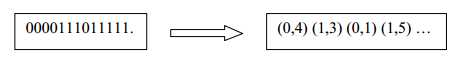
\includegraphics[scale=1]{run-length_encoding.png}
				\caption{Algoritmo di compressione Run-Length Encoding.}
				\label{fig:run-length_encoding}
			\end{figure}
			
		\subsection{Move-To-Front} \label{subsec:move-to-front}
			
			La codifica \textit{Move-To-Front} (o \textit{MTF}) si basa sul concetto di entropia ed infatti è ottimizzata quando la lettura di un carattere aumenta le probabilità di trovare lo stesso carattere subito dopo.\\
			L'algoritmo inizia codificando le lettere dell'alfabeto secondo l'ordine usuale (da 0 a 25). Quindi ogni carattere che viene incontrato viene spostato in cima alla lista. In generale, elementi in cima alla lista vengono codificati con meno bit, mentre quelli verso il fondo richiedono più bit.\\
			\\
			Se ad esempio prendiamo la parola ``BANANAAA'', la codifica MTF di questa parola sarà quella in Tabella \ref{tab:move-to-front}.
			
			\begin{table}[h!]
				\centering
				\begin{tabular}{|l|l|c|}
					\multicolumn{1}{c}{\textbf{Sequenza}} & \multicolumn{1}{c}{\textbf{Codifica}} & \multicolumn{1}{c}{\textbf{Lista}}\\
					\hline
					b & 1 & abcdefghijklmnopqrstuvwxyz\\
					\hline
					ba & 1, 1 & bacdefghijklmnopqrstuvwxyz\\
					\hline
					ban & 1, 1, 13 & abcdefghijklmnopqrstuvwxyz\\
					\hline
					bana & 1, 1, 13, 1 & nabcdefghijklmopqrstuvwxyz\\
					\hline
					banan & 1, 1, 13, 1, 1 & anbcdefghijklmopqrstuvwxyz\\
					\hline
					banana & 1, 1, 13, 1, 1, 1 & nabcdefghijklmopqrstuvwxyz\\
					\hline
					bananaa & 1, 1, 13, 1, 1, 1, 0 & anbcdefghijklmopqrstuvwxyz\\
					\hline
					bananaaa & 1, 1, 13, 1, 1, 1, 0, 0 & anbcdefghijklmopqrstuvwxyz\\
					\hline
				\end{tabular}
				\caption{Algoritmo di compressione Move-To-Front.}
				\label{tab:move-to-front}
			\end{table}
		
		\subsection{Codifica di Huffman} \label{subsec:codifica_huffman}
			
			Il concetto di entropia viene ampiamente applicato anche alla codifica di Huffman che, come vedremo più avanti, viene utilizzata all'interno dell'algoritmo di compressione MP3. L'idea che sta alla base della codifica di Huffman è quella di codificare con meno bit i caratteri più frequenti. La probabilità di incontrare determinati caratteri dev'essere determinata a priori (ad esempio analizzando i dati che si vogliono comprimere). Successivamente, in base alle probabilità calcolate, si assegnano codifiche più corte ai caratteri più frequenti e si memorizzano le associazioni carattere-codifica in una tabella, detta \textit{tabella di Huffman}, necessaria per la successiva decodifica dei dati. Come possiamo vedere in Figura \ref{fig:huffman}, la tabella di Huffman può essere rappresentata anche come un albero binario.
			
			\begin{figure}[h!]
				\centering
					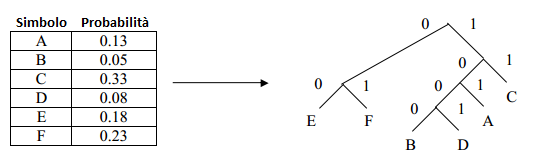
\includegraphics[scale=1]{huffman.png}
				\caption{Codifica di Huffman.}
				\label{fig:huffman}
			\end{figure}
		
	\chapter{Pianificazione delle attività}

Il progetto consiste nel valutare da un punto di vista temporale i risultati degli esperimenti eseguiti con Snort. Per fare questo abbiamo utilizzato due macchine con OS Ubuntu 12.04 su cui, seguendo i passi descritti nel capito successivo, abbiamo installato e opportunamente configurato Snort come IDS. Il sistema alla base delle analisi quindi si compone di una prima macchina che avrà funzione di sistema da difendere (nodo A) ed una seconda con la funzione di attaccante (nodo B) collegate ad una rete wifi locale.
La necessità di eseguire Snort su entrambe le componenti del sistema è legata alla necessità di dover tracciare i tempi d'invio, d'iniezione e d'individuazione delle operazioni di fault injection. In pratica, nel nodo A Snort provvederà sia a loggare tutto il traffico diretto verso se stesso dal nodo B, sia a generare gli alert dovuti agli attacchi individuati, mentre nel nodo B provvederà a loggare tutti i pacchetti diretti da B ad A, così da tracciare i tempi d'invio degli attacchi. I codici relativi alle regole Snort che sono state scritte per permettere ai due nodi di fare sia da Packet Sniffer che da Packet Logger possono essere trovati nell'Appendice A, Codici \ref{lst:attaccante} e \ref{lst:ids}.\\
Il sistema di misura si compone quindi dei due file di log generati rispettivamente sui due nodi che, assieme all'output dei software usati per generare la fault injection, permettono di registrare tutta la storia temporale degli attacchi al fine di verificare l'azione delle regole di Snort.\\
Purtroppo, in un primo momento di analisi del problema e di sperimentazione, ritenevamo sufficiente loggare soltanto i pacchetti in entrata ed in uscita, rispettivamente, nel nodo A e dal nodo B. Soltanto in fase di analisi ci siamo resi conto che, senza il flusso di dati in entrambe le direzioni ed in entrambi i nodi, alcune misure (come ad esempio la durata totale dell'attacco) non potevano essere calcolate correttamente. Per ragioni di tempistiche, abbiamo deciso di mantenere gli esperimenti e i relativi log così com'erano, precisando comunque che alcune misure, per questo motivo, sono state approssimate e consci del fatto che un'applicazione più rigida della metodologia di testing avrebbe richiesto la ripetizione di tutti gli esperimenti con le nuove specifiche.

\begin{figure}[h!]
	\centering
	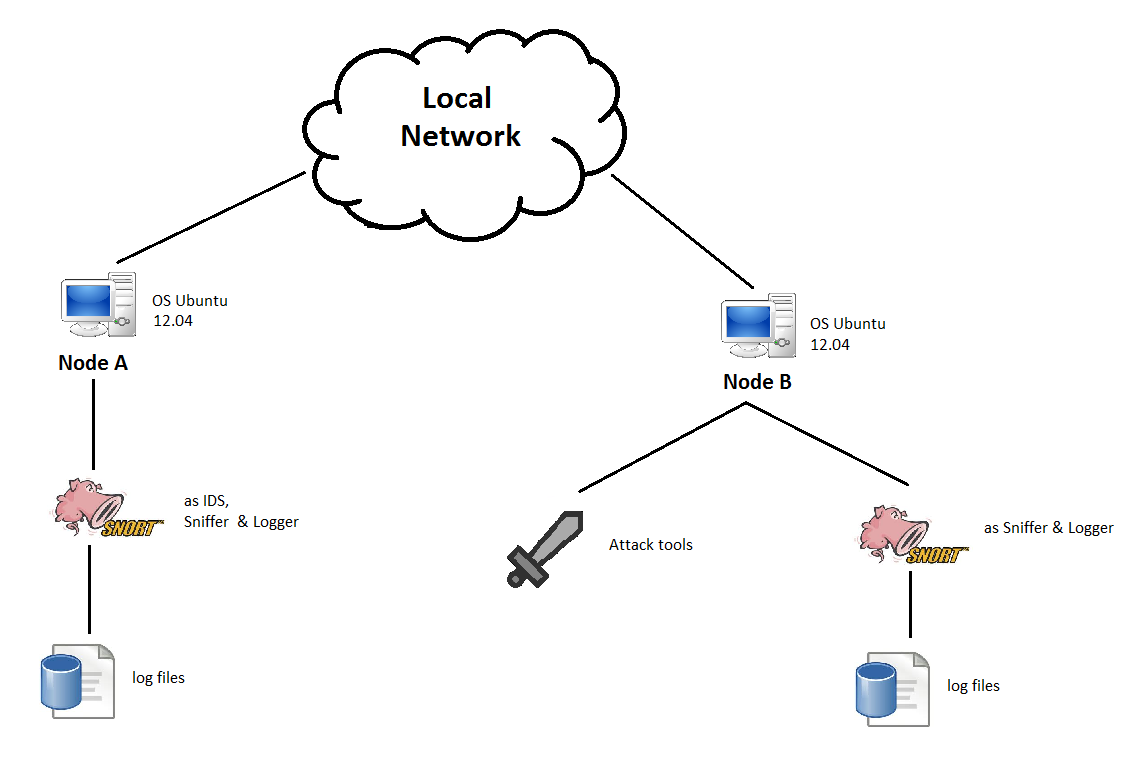
\includegraphics[scale=0.5]{figure/schema.png}
	\caption{Schema della configurazione utilizzata nei vari esperimenti.}
\end{figure}

\section{Sfasamento dei clock}

Il ``semplice'' sistema di misura brevemente descritto in precedenza deve però tenere conto del problema dello sfasamento dei clock sulle due macchine, è infatti errato assumere che entrambe abbiano la stessa visione del tempo che è appunto governata dal clock interno a ciascuna macchina. Inoltre, anche se in un certo istante il clock delle due macchine segnasse lo stesso valore, non è detto che questo valga sempre: è infatti possibile che i due clock si allontanino o si avvicinino durante il tempo, rendendo impossibile fare qualsiasi stima di natura statica.\\
Per fare sì che i tempi registrati nel nodo A siano consistenti a quelli registrati nel nodo B è necessario mettere in piedi un processo di sincronizzazione. Un protocollo utile per, parzialmente, risolvere il problema è il Network Time Protocol, in sigla NTP, un protocollo per la sincronizzazione degli orologi di computer all'interno di una rete a commutazione di pacchetto.\\
Come prima cosa quindi è necessario scaricare ed installare su entrambe le macchine il pacchetto \textit{ntp} che mette a disposizione varie funzionalità per la sincronizzazione.\\
Un primo approccio può fare uso del comando \textbf{ntpd}, il quale mette in esecuzione un processo \textit{demone} che in \textit{background} provvede a sincronizzare l'orologio di sistema con quello di un server opportunamente specificato nel file (\textit{/etc/ntp.conf}). Questo approccio ha però due problemi: richiede alcune ore per arrivare a registrare una buona approssimazione del tempo del server e continuando la sua esecuzione in background e in modo asincrono rispetto all'altra macchina che compone il sistema può andare a modificare la visione del tempo di una macchina durante l'esecuzione di un'esperimento rischiando di produrre inconsistenze tra i dati raccolti.
Per fornire evidenza di questa situazione riportiamo qui di seguito due frammenti di log relativi al nodo A e al nodo B durante un esperimento di fault injection (alcuni dettagli non rilevanti sono stati omessi per una maggiore chiarezza di lettura):

\begin{center}
	\textbf{Nodo A:}
	\begin{tabular}{|c|c|c|c|c|}
	\hline
	TIMESTAMP & MSG & PROTOCOL & FROM\_IP & TO\_IP\\
	\hline
	07/09-17:38:37.271491 & ICMP PING BSDtype&	ICMP&	192.168.137.170&		192.168.137.180\\
	\hline
	07/09-17:38:37.271491& 		ICMP PING *NIX&	ICMP&	192.168.137.170	&	192.168.137.180\\
	\hline
	07/09-17:38:37.271491 &	PACKET RECEIVED&	ICMP&	192.168.137.170&		192.168.137.180\\
	\hline
	07/09-17:38:37.271491 &	ICMP PING&	ICMP&	192.168.137.170&		192.168.137.180\\
	\hline
	07/09-17:38:37.271544&	ICMP Echo Reply&	ICMP&	192.168.137.180&		192.168.137.170\\
	\hline
	07/09-17:38:38.194984 &	ICMP PING BSDtype	& ICMP&	192.168.137.170&		192.168.137.180\\
	\hline
	07/09-17:38:38.194984 &	ICMP PING *NIX&	ICMP&	192.168.137.170&		192.168.137.180\\
	\hline
	07/09-17:38:38.194984 &	PACKET RECEIVED&	ICMP&	192.168.137.170&		192.168.137.180\\
	\hline
	07/09-17:38:38.194984 &	ICMP PING&	ICMP&	192.168.137.170&		192.168.137.180\\
	\hline
	07/09-17:38:38.195038 &	ICMP Echo Reply	& ICMP&	192.168.137.180&		192.168.137.170\\
	\hline
	07/09-17:38:39.116375 &	ICMP PING BSDtype&	ICMP&	192.168.137.170&		192.168.137.180\\
	\hline
	07/09-17:38:39.116375 &	ICMP PING *NIX&	ICMP&	192.168.137.170&		192.168.137.180\\
	\hline
	07/09-17:38:39.116375 &	PACKET RECEIVED&	ICMP&	192.168.137.170&		192.168.137.180\\
	\hline
	07/09-17:38:39.116375 &	ICMP PING&	ICMP&	192.168.137.170&		192.168.137.180\\
	\hline
	07/09-17:38:39.116406 &	ICMP Echo Reply&	ICMP&	192.168.137.180&		192.168.137.170\\
	\hline
	07/09-17:38:40.140671 &	ICMP PING BSDtype&	ICMP&	192.168.137.170&		192.168.137.180\\
	\hline
	07/09-17:38:40.140671 &	ICMP PING *NIX&	ICMP&	192.168.137.170&		192.168.137.180\\
	\hline
	07/09-17:38:40.140671&	PACKET RECEIVED&	ICMP&	192.168.137.170	&	192.168.137.180\\
	\hline
	07/09-17:38:40.140671 &	ICMP PING&	ICMP&	192.168.137.170&		192.168.137.180\\
	\hline
	07/09-17:38:40.140727 &	ICMP Echo Reply&	ICMP&	192.168.137.180	&	192.168.137.170\\
	\hline
	07/09-17:38:47.513307 	&	PACKET RECEIVED&	TCP&	192.168.137.170&	192.168.137.180\\
	\hline
	\end{tabular}
\end{center}
\clearpage
\begin{center}
	\textbf{Nodo B:}
	\begin{tabular}{|c|c|c|c|c|}
	\hline
	TIMESTAMP & MSG & PROTOCOL & FROM\_IP & TO\_IP\\
	\hline
	07/09-17:38:37.128073&	ICMP PING BSDtype&	ICMP&	192.168.137.170	&	192.168.137.180\\
		\hline
	07/09-17:38:37.128073 &	ICMP PING *NIX&	ICMP&	192.168.137.170	&	192.168.137.180\\
		\hline
	07/09-17:38:37.128073 &	PACKET SENT&	ICMP&	192.168.137.170	&	192.168.137.180\\
		\hline
	07/09-17:38:37.128073 &	ICMP PING&	ICMP&	192.168.137.170	&	192.168.137.180\\
		\hline
	07/09-17:38:37.320961 &	ICMP Echo Reply	& ICMP&	192.168.137.180	&	192.168.137.170\\
		\hline
	07/09-17:38:38.129178 &	ICMP PING BSDtype&	ICMP&	192.168.137.170&		192.168.137.180\\
		\hline
	07/09-17:38:38.129178 &	ICMP PING *NIX&	ICMP&	192.168.137.170	&	192.168.137.180\\
		\hline
	07/09-17:38:38.129178 &	PACKET SENT&	ICMP&	192.168.137.170	&	192.168.137.180\\
		\hline
	07/09-17:38:38.129178 &	ICMP PING&	ICMP&	192.168.137.170	&	192.168.137.180\\
		\hline
	07/09-17:38:38.243095 &	ICMP Echo Reply&	ICMP&	192.168.137.180	&	192.168.137.170\\
		\hline
	07/09-17:38:39.130354 &	ICMP PING BSDtype&	ICMP&	192.168.137.170&		192.168.137.180\\
		\hline
	07/09-17:38:39.130354 &	ICMP PING *NIX&	ICMP&	192.168.137.170&		192.168.137.180\\
		\hline
	07/09-17:38:39.130354 	&	PACKET SENT&	ICMP&	192.168.137.170	&	192.168.137.180\\
		\hline
	07/09-17:38:39.130354 	&	ICMP PING&	ICMP&	192.168.137.170	&	192.168.137.180\\
		\hline
	07/09-17:38:39.163513 &	ICMP Echo Reply&	ICMP&	192.168.137.180	&	192.168.137.170\\
		\hline
	07/09-17:38:40.131860 &	ICMP PING BSDtype&	ICMP&	192.168.137.170	&	192.168.137.180\\
		\hline
	07/09-17:38:40.131860 &	ICMP PING *NIX&	ICMP&	192.168.137.170	&	192.168.137.180\\
		\hline
	07/09-17:38:40.131860 &	PACKET SENT	& ICMP&	192.168.137.170&		192.168.137.180\\
		\hline
	07/09-17:38:40.131860 &	ICMP PING&	ICMP&	192.168.137.170	&	192.168.137.180\\
		\hline
	07/09-17:38:40.190195 	&	ICMP Echo Reply&	ICMP&	192.168.137.180	&	192.168.137.170\\
		\hline
	07/09-17:38:47.564978 &	PACKET SENT&	UDP&	192.168.137.170&	192.168.137.1\\
		\hline
	\end{tabular}
\end{center}

Osservando i tempi d'invio ed i tempi di recezione dei messaggi si può facilmente notare come per i primi pacchetti i tempi di recezione, come ci si può aspettare, siano maggiori dei tempi d'invio mentre questo non vale dal quinto pacchetto in poi dove i tempi di recezione risultano improvvisamente minori dei tempi d'invio. Questa inconsistenza può essere frutto di una sincronizzazione dell'orologio di una delle due macchine per mezzo del demone generato con il comando \textit{ntpd} o anche uno sfasamento dei clock. La possibilità d'occorrenza di questa situazione rende quindi impossibile dare confidenza sui risultati ottenuti a causa della variabilità della visione temporale, di una o di entrambe le macchine, durante l'esecuzione di un esperimento.\\
Questo problema può essere risolto utilizzando altri due comandi. Sarà infatti necessario disattiva il servizio \textit{ntp} eliminando il problema della sincronizzazione degli orologi asincrona tra le due macchine, utilizzando il comando \textit{service ntp stop}. Successivamente dopo l'esecuzione di ogni esperimento sarà necessario utilizzare il comando \textit{ntpdate}, il quale permette di sincronizzare l'orologio e ricevere l'offset di aggiustamento applicato. Utilizzando quest'offset che corrisponde ad una stima dell'errore temporale commesso da ciascuna macchina, durante l'esecuzione dell'esperimento, possiamo cercare di "correggere" le misure registrate. Ad esempio se l'offset resitutito da \textit{ntpdate} sul nodo A è +2ms mentre l'offset restituito sul nodo B è -4ms, si può cercare di correggere le misure registrate sul nodo A e sul nodo B rispettivamente sommando e sottraendo tali offset.
Questa correzione naturalmente non elimina totalmente l'errore sistematico commesso, in quanto gli offset sono stime dell'errore, ma si riesce comunque a limitare l'errore di misurazione.
Quindi il sistema di misura introdotto avrà come riferimento l'orologio (il clock) del server utilizzato con il comando \textit{ntpdate}, la procedura di misura consisterà nell'effettuare il \textit{timestamp} di ogni pacchetto inviato/ricevuto con una risoluzione di \textit{$10^{-6}$s} ed un'intrusività trascurabile per la risoluzione apprezzata. Ad ognuno di questi tempi sarà poi sommato/sottratto l'offset tra il tempo macchina e il tempo del server riscontrato durante l'esperimento.



	
\chapter{Instrumentazione del sistema}
	
	\section{Installazione e configurazione di Snort}
		
		Il progetto consiste nel valutare il comportamento, dal punto di vista temporale, di Snort come IDS. Andremo ad installare Snort in due macchine che utilizzano come OS Ubuntu 12.04.\\
		Per installare e configurare Snort come IDS è necessario seguire i seguenti passi:
		\begin{itemize}
		  \item \textbf{Scaricare librerie necessarie a Snort}: dobbiamo cioè verificare se nel nostro sistema sono già installate librerie come: libpcap0.8, libpcre3, libdnet-1.12, daq-1.1.1, flex, libpcap-ruby, libtool.
		  \item \textbf{Scaricare la versione aggiornata di Snort} dal sito \textit{http://www.snort.org/\\ snort-downloads} e procediamo con l'installazione vera e propria del software.
		  \item \textbf{Aprire il prompt}, ed eseguire in successione i comandi:
		        \begin{itemize}
		            \item \textit{sudo tar zxvf snort-2.9.4.6.tar.gz}
		            \item \textit{cd snort-2.9.4.6}
		            \item \textit{sudo ./configure --prefix=/usr/local/snort --enable-sourcefire}
		            \item \textit{sudo make}
		            \item \textit{sudo make install}
		            \item \textit{sudo mkdir /var/log/snort}
		            \item \textit{sudo chown snort:snort /var/log/snort}
		        \end{itemize}
		  \item \textbf{Scaricare il file delle regole}: per fare questo eseguiamo i comandi:
		        \begin{itemize}
		            \item \textit{sudo tar zxvf snortrules-snapshot-2946.tar.gz -C /usr/local/snort}
		            \item \textit{sudo mkdir /usr/local/snort/lib/snort\_dynamicrules}
		            \item \textit{sudo cp /usr/local/snort/so\_rules/precompiled/Ubuntu-10-4/i386/2.9.4.6/* /\\ /usr/local/snort/lib/snort\_dynamicrules}
		            \item \textit{sudo touch /usr/local/snort/rules/white\_list.rules}
		            \item \textit{sudo touch /usr/local/snort/rules/black\_list.rules}
		            \item \textit{sudo ldconfig}
		        \end{itemize}
		  \item \textbf{Configurare Snort}: dobbiamo modificare il file di configurazione \textit{snort.conf} eseguendo il comando \textit{sudo gedit /usr/local/snort/etc/snort.conf} e modificare le righe:
		        \begin{itemize}
		            \item \textit{var WHITE\_LIST\_PATH ../rules} e \textit{var BLACK\_LIST\_PATH ../rules} rispettivamente in \textit{var WHITE\_LIST\_PATH /usr/local/snort/rules} e \textit{var BLACK\_LIST\_PATH /usr/local/snort/rules}
		            \item \textit{dynamicpreprocessor directory /usr/local/lib/snort\_dynamicpreprocessor/},\\ \textit{dynamicengine /usr/local/lib/snort\_dynamicengine/libsf\_engine.so} e \\ \textit{dynamicdetection directory /usr/local/lib/snort\_dynamicrules} rispettivamente in \\ \textit{dynamicpreprocessor directory /usr/local/snort/lib/snort\_dynamicpreprocessor/},\\ \textit{dynamicengine /usr/local/snort/lib/snort\_dynamicengine/libsf\_engine.so} e \\ \textit{dynamicdetection directory /usr/local/snort/lib/snort\_dynamicrules}
		        \end{itemize}
		        ed aggiungere nella sezione relativa ai file di output generati, la riga \textit{output alert\_csv: alert.csv default} per far si che il report generato sia già in formato csv (ci tornerà utile in fase di analisi).
		  \item \textbf{Lanciare Snort come IDS}: per lanciare Snort come IDS è necessario eseguire il comando snort come root e specificare:
		      \begin{itemize}
		        \item la rete che s'intende monitorare, per mezzo dell'opzione \textit{-i} seguita dal nome della rete (ad esempio \textit{wifi0} per la rete wifi);
		        \item la richiesta di riportare anche su terminale i pacchetti che trafficano nella rete, usando l'opzione \textit{-dev};
		        \item il percorso in cui Snort andrà a salvare il report degli alert rilevati, usando l'opzione \textit{-l} seguita appunto dal percorso;
		        \item il percorso in cui Snort può trovare il proprio file di configurazione, usando l'opzione \textit{-c} seguita dal percorso.
		      \end{itemize}
		\end{itemize}
		
		Snort è stato così installato e ben configurato su entrambe le macchine che andranno a comporre il sistema su cui faremo l'analisi temporale richiesta.
		
	\section{Tool di fault injection}
	In questa sezione descriviamo le caratteristiche e le opzioni dei vari tool utilizzati per gli esperimenti di fault injection, questi tool dovranno essere installati sulla macchina che svolgerà il ruolo di attaccante (nodo B).
	
	\subsection{NMap}
	Nmap ("Network Mapper") è uno strumento open source per la network exploration e l'auditing. \'E stato progettato per scansionare rapidamente reti di grandi dimensioni, ma è indicato anche per l'utilizzo verso singoli host. Nmap usa pacchetti IP raw (grezzi, non formattati) in varie modalità per determinare quali host sono disponibili su una rete, che servizi (nome dell'applicazione e versione) vengono offerti da questi host, che sistema operativo (e che versione del sistema operativo) è in esecuzione, che tipo di firewall e packet filters sono usati, e molte altre caratteristiche.
	L'output di Nmap è uno scan di un elenco di obiettivi, con informazioni supplementari per ognuno a seconda delle opzioni usate. Tra queste informazioni è vitale la ``tabella delle porte interessanti''. Questa tabella elenca il numero della porta e il protocollo, il nome del servizio, e il suo stato attuale.  La tabella delle porte può anche includere dettagli quali le versioni dei software disponibili se è stata usata l'opzione appropriata.\\
	Installare \textit{nmap} è semplicissimo: sarà sufficiente digitare il comando \textit{sudo apt-get install nmap} sul terminale.\\
	Negli esperimenti abbiamo scelto di valutare il comportamento di Snort soggetto ad attacchi generati con \textit{nmap} e le seguenti opzioni:
	\begin{itemize}
	    \item \textit{ --osscan\_guess (Guess OS detection results)}, con questa opzione attiva se nmap non è in grado di rilevare una corrispondenza esatta dell'OS, propone come possibilità gli OS più vincini alla rilevazione.\\ La corrispondenza però deve essere molto simile perchè Nmap lo faccia per default. Entrambe queste opzioni (equivalenti) fanno si che Nmap proceda con il riconoscimento dell'OS in modo più aggressivo.
	    \item \textit{--version\_light (Attiva la modalità Light)}, questa modalità rende il Version Scanning drasticamente più veloce, riducendone però la capacità di identificare accuratamente i servizi.
	    \item \textit{--version\_all (Prova ogni singolo pacchetto-sonda)},questa opzione assicura che ogni singolo pacchetto-sonda venga utilizzato su ogni singola porta.
	    \item \textit{-T (Imposta un template di temporizzazione)}, tramite questa opzione nmap offre un approccio per il testing più semplice, lo fa mediante sei "timing templates", ovvero opzioni pre-impostate per regolare l'aggressività della scansione. Esse si specificano mediante l'opzione -T seguita dal numero del template
	           corrispondente o dal suo nome. Essi sono: paranoico (0), furtivo (1), educato (2), normale (3), aggressivo (4) e folle (5). I primi due vengono usati per evitare i sistemi anti-intrusione (IDS). La modalità "gentile" rallenta la scansione in modo da usare meno banda e risorse sulla macchina bersaglio. La modalità  "normale" è di default (e pertanto l'opzione -T3 non modifica nulla). La modalità "aggressiva" incrementa la velocità assumendo che si è su una rete veloce ed affidabile. Infine la modalità "folle" dà per scontato che si è su una rete estremamente veloce ed affidabile o che si vuole sacrificare l'accuratezza in nome della velocità.
	
	    \item \textit{-A (Opzioni di scan aggressive)}, questa opzione abilita opzioni addizionali avanzate e aggressive.
	
	    \item \textit{-sn}, esegue una scansione ping ed esclude la scansione sulle porte.\\Questo comando è stato testato, tra i vari esperimenti condotti in questo lavoro, ma non è stato rilevato in alcun modo da Snort, né sotto forma di alert né come pacchetti ricevuti. Quindi questo particolare attacco è stato escluso nella fase di analisi.
	
	
	\end{itemize}
	
	\subsection{Ping}
	Ping verifica le connessioni a computer remoti. Invia pacchetti di echo ICMP Internet Control Message Protocol a un computer e attende i pacchetti di risposta. Ping attende di default fino a 1 secondo per ogni pacchetto inviato e viene stampato il numero di pacchetti trasmessi e ricevuti sulla console. L'attesa per ogni pacchetto inviato essere specificata utilizzando l'opzione \textit{-i}
	Il comando \textit{ping} è già disponibile all'interno della distribuzione Ubuntu utilizzata.\\
	Per i nostri esperimenti andremo ad utilizzare l'opzione \textit{-i} del comando, tale opzione permette di esplicitare l'intervallo di tempo da attendere tra l'invio di ogni pacchetto. Il valore di default è un secondo, o non attendere in modalità \textit{flood}. Solo un super-utente può impostare l'intervallo  a valori inferiori di 0,2 secondi.\\
	Per verificare la variazione di funzionamento di Snort a seguito di pacchetti inviati più velocemente abbiamo creato una nuova regola:\\
	\\
	\textit{alert icmp any any -> 192.168.137.180 any (msg:``TOO MUCH PING''; threshold: type both, track by\_src, count 10, seconds 3; classtype:attempted-dos; sid:51000; rev:2;)}\\
	\\	
	Tale regola ci permette di discriminare il comportamento tenuto da Snort al variare del valore per l'opzione \textit{-i}.
	
	
	\subsection{Metasploit}
	Metasploit Project è un progetto open source (rilasciato con licenza BSD) dedicato alla sicurezza informatica il quale fornisce informazioni sulle vulnerabilità della rete e ne semplifica le operazioni di penetration testing e ne aiuta nello sviluppo di sistemi di rilevamento di intrusioni.
	Assieme al progetto Metasploit troviamo anche Metasploit Framework uno strumento dedicato principalmente allo sviluppo e l'esecuzione di exploit ai danni di una macchina remota.
	Sono messe a disposizioni varie interfaccie ma nel seguito andremo ad utilizzare l'interfaccia web msfweb, utile per usare il framework con tutta la comodità di un'interfaccia web.
	Metasploit Project viene rilasciato con un semplice installar il quale ci permetterà d'installare l'applicazione in qualsiasi distribuzione Linux.
	Per installare Metasploit Project su OS Ubuntu basta digitare:
	\begin{itemize}
	\item \textit{wget http://downloads.metasploit.com/data/releases/metasploit-latest-linux-installer.run}
	\item \textit{chmod +x metasploit-latest-linux-installer.run}
	\item \textit{sudo ./metasploit-latest-linux-installer.run}
	\end{itemize}
	a questo punto si aprirà un wizard con il quale procederemo all'installazione di Metasploit e in cui ci verrà chiesto d'inserire la porta SSL dedicata al servizio e successivamente la creazione dei certificati SSL.\\
	Al termine del Wizard d'installazione potremo accedere alla Web Ui di Metasploit la qual ci confermerà la corretta installazione. Potremo a questo punto lanciare l'interfaccia web di Metasploità dove sarà richiesto di creare ed attivare un account.\\
	Per i nostri esperimenti si è scelto di utilizzare \textit{metasploit} come \textit{port scan}, sarà necessario digatere l'indirizzo ip su cui eseguire la scansione e successivamente specificare le varie opzioni avanzate per la scansione. Le scansioni che effettueremo sono essenzialmente due, quella di default senza specificare alcuna opzione avanzata e una seconda in cui abiliteremo la \textit{Scan SNMP community strings Information}: quest'opzione lancia un task in background per analizzare i device SNMP che corrispondono ad una serie di stringhe (essendo un lavoro generalmente lungo, viene eseguito in parallelo con le altre scansioni base).
	
	\subsection{Traceroute}
	\textit{Traceroute} cerca di tracciare il percorso seguito dai pacchetti IP per un qualche host internet. Cerca i passaggi intermedi, lanciando pacchetti sonda con un piccolo TTL, e quindi resta in ascolto di un \textit{ICMP reply} da un router intermedio. \textit{Traceroute} inizia la rilevazione con un TTL di uno, e lo incrementa fino a quando viene ricevuto un \textit{ICMP port unreachable reply}. Questo significa che la sonda o ha raggiunto l'host, o ha raggiunto il TTL massimo.\\
	Per rendere disponibile questo tool, se non già presente tra le librerie dell'OS, è necessario eseguire il comando \textit{apt-get install traceroute} tramite il quale sarà installato e quindi reso disponibile.\\
	Negli esperimenti andremo ad attivare alternativamente le seguenti opzioni:
	\begin{itemize}
	    \item \textit{-I (icmp)}, abilita il comportamento ad ora usuale per traceroute, utilizzando pacchetti ICMP ECHO per le sonde.
	    \item \textit{-T (tcp)}, abilita un nuovo comportamento per traceroute destinato ad aggirare i firewall.\\ Utilizza una porta di destinazione costante (di default è 80, http).\\
	        Questo metodo utilizza la ben nota "\textit{half-open technique}", che impedisce alle applicazioni sull'host di destinazione di far vedere le nostre sonde a tutti.\\
	        Includendo l'opzione -T all'attacco con traceroute, Snort rileva (sul nodo A) una serie di pacchetti in arrivo ma non genera alcun tipo ti alert (o perché l'attacco viene considerato innocuo, o perché Snort non ha regole sufficienti a rilevarlo). Nella fase di analisi, quindi, sono state escluse le misurazioni sui tempi di detection che riguardano quest'esperimento.
	
	    \item \textit{-N (squeries)}, Specifica il numero di pacchetti sonda inviati simultaneamente.\\
	    L'invio di più sonde contemporaneamente può accelerare notevolmente traceroute (il valore predefinito è 16). Si noti che alcuni router e gli host possono utilizzare \textit{ICMP  rate  throttling}e in una tale situazione specificando un numero troppo grande si può avere la perdita di alcune risposte.
	\end{itemize}
	
	\section{Tool di data integration e analisi}
	In questa ultima sezione andiamo a descrivere il tool che utilizzeremo per integrare e manipolare i dati raccolti al fine di generare successivamente un sistema OLAP su cui effettuare tutte le analisi.\\
	Il framework utilizzato è \textit{Pentaho}, precisamente il tool \textit{Kettle} per la \textit{Data Integration} ed il motore MOLAP \textit{Mondrian} per analisi di tipo OLAP.\\
	Il framework messo a disposizione da Pentaho permette di sviluppare soluzioni complete per la \textit{Business Intelligence} ma noi ci limiteremo ad utilizzare i tool sopra citati, che sono ampiamente sufficienti per soddisfare le nostre richieste.\\
	Utilizzando il tool \textit{Kettle}, è possibile integrare e manipolare i file \textit{.csv} generati in fase sperimentale, così da renderli in una forma più consona alla memorizzazione all'interno di un database, ad esempio sarà possibile dividere il campo relativo al timestamp nelle sue sottocomponenti, così da rendere più semplice la correzione del tempo indicata dall'offset di sfasamento degli orologi rilevato tramite il comando \textit{ntpdate} oppure ancora permette di aggiungere nuovi campi come ad esempio ``EXP\_ID'' che andrà a identificare univocamente i pacchetti relativi ad un determinato esperimento.
	Vediamo qui la trasformazione (per comodità divisa in quattro immagini) che permetterà di integrare tra loro i dati relativi ai vari esperimenti eseguiti:
	
	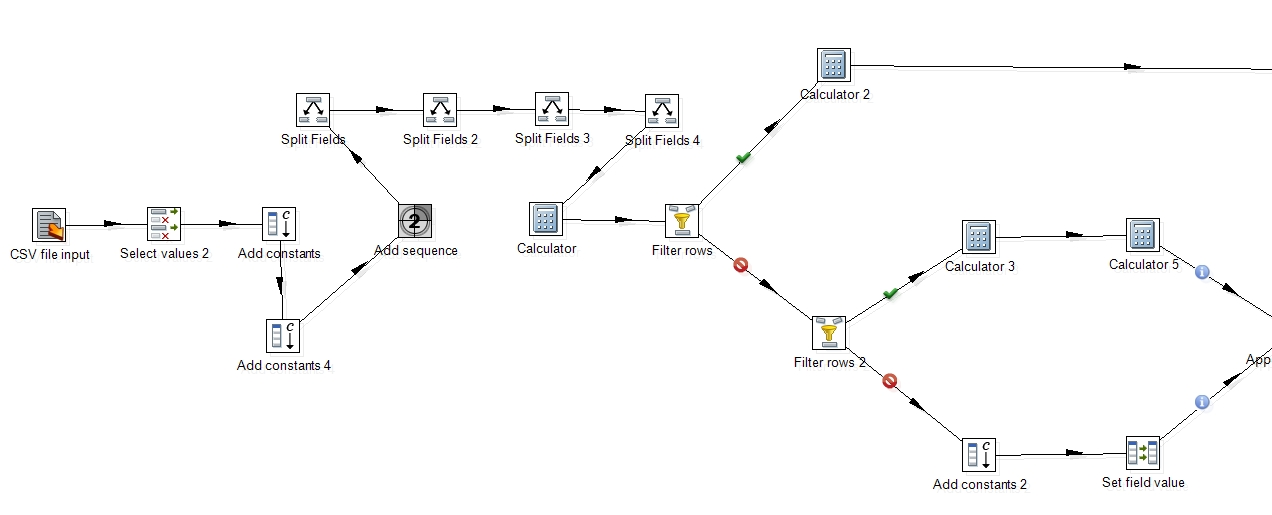
\includegraphics[scale=0.4]{figure/kettle1.jpg}\\
	
	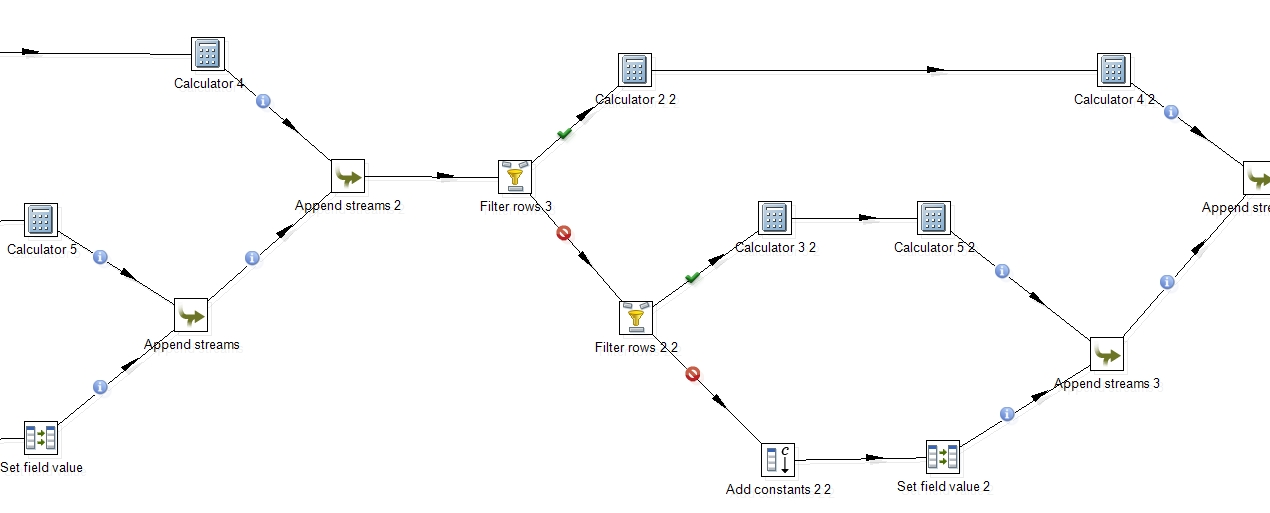
\includegraphics[scale=0.4]{figure/kettle2.jpg}\\
	
	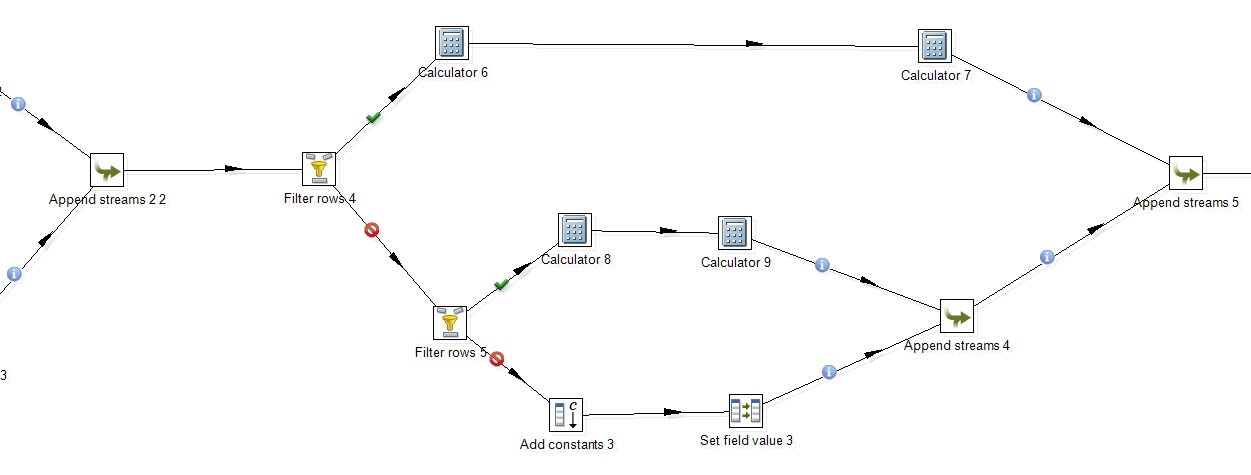
\includegraphics[scale=0.4]{figure/kettle3.jpg}\\
	
	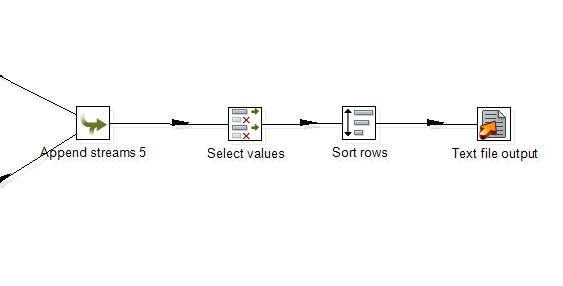
\includegraphics[scale=0.4]{figure/kettle4.jpg}
	
	Il file generato da Kettle (file di log \textit{logCompleto.csv}), ancora in formato \textit{.csv}, consisterà nell'elenco di tutti i pacchetti loggati a cui sono associate tutte le informazioni registrate durante gli esperimenti. Ovviamente tale file è spesso e volentieri ridondante, proprio come chiede la logica OLAP.\\
	A questo punto utilizzando il tool \textit{Mondrian} è possibile definire uno \textit{star-schema}, che avrà la struttura indicata in Figura \ref{fig:star}.
	
	\begin{figure}[h!]
		\centering
		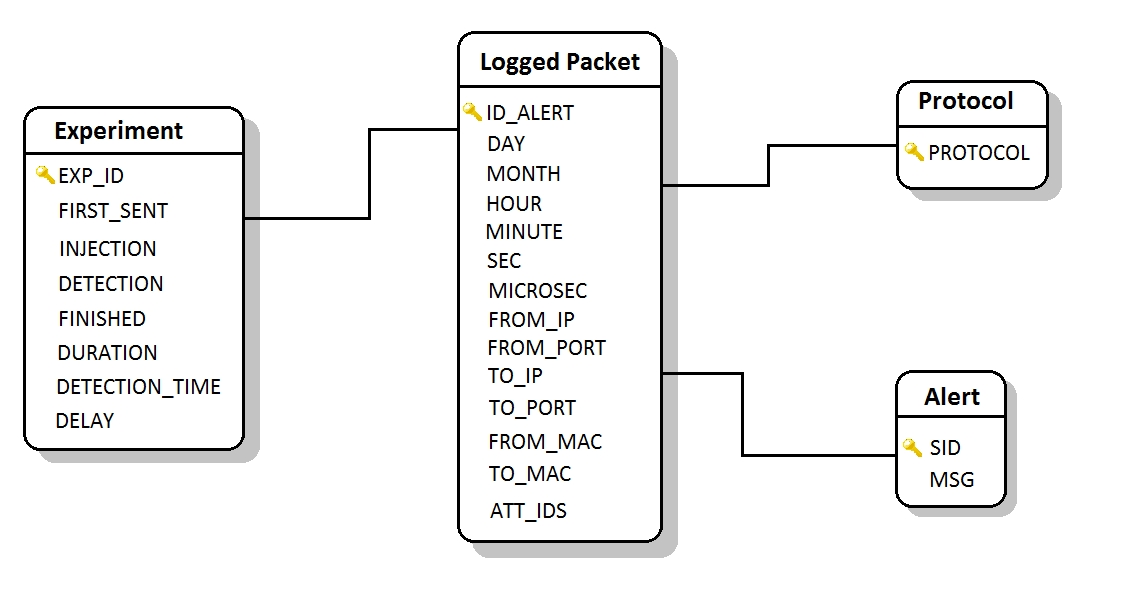
\includegraphics[scale=0.45]{figure/star-schema.jpg}
		\caption{\textit{Schema a stella} costruito sul file di log finale.}
		\label{fig:star}
	\end{figure}
	
	Questa struttura ci permetterà di modellare il fatto "\textit{Logged Packet}". L'analisi, infatti, è volta ad analizzare come Snort reagisce e varia le proprie prestazioni al variare sia di tool di fault injection che, pur rimanendo all'interno dello stesso tool, delle opzioni attive.\\
	Prima di caricare nel database tutte le informazioni contenute nel file \textit{.csv}, per velocizzare il processo di analisi utilizzeremo un semplice programma \textit{Java} (Codice \ref{lst:java}, Appendice A), il quale, analizzando il file generato da \textit{Kettle}, permetterà di calcolare le seguenti tempistiche necessarie per l'analisi:
	\begin{itemize}
	    \item L'istante di tempo in cui l'attacco è generato dal nodo B.
	    \item L'istante di tempo in cui l'attacco è iniettato sul nodo A.
	    \item L'istante di tempo in cui l'attacco è individuato da parte di Snort.
	    \item Il ritardo di trasmissione introdotto dalla rete.
	    \item Il tempo di \textit{detection}, cioè il tempo impiegato da Snort per rilevare l'attacco.
	    \item La durata dell'attacco.
	\end{itemize}
	
	Questi tempi, per una più semplice manipolazione, saranno ``assoluti'' cioè si riferiranno ad uno stesso giorno di uno stesso mese e l'orario sarà espresso in microsecondi. Ogni esperimento avrà ovviamente proprie tempistiche.\\
	Arrivati a questo punto tutti i dati raccolti e le quantità necessarie per l'analisi saranno nella forma più adatta per la memorizzazione in un database (file di log \textit{logFinale.csv}). Procederemo con l'analisi per mezzo di funzioni OLAP rese disponibili anch'esse nel framework \textit{Pentaho}, precisamente usando \textit{Mondrian}. Sarà così semplice fornire grafici o report di ogni tipo incrociando a piacimento i dati raccolti per i vari esperimenti.
	Riporteremo le analisi effettuate nei seguenti capitoli. Occorre però osservare che il numero di comparazioni effettuabili sono molteplici e tutte facilmente ottenibili utilizzando \textit{Pentaho}, sfruttando la ridondanza creata per mezzo di \textit{kettle} nel file \textit{.csv} che svolge la funzione di repositary dei dati sperimentali.

	\chapter{Analisi temporale}

\section{Nmap}
In questo capitolo vengono presentati i risultati della comparazione tra le varie istanze di esecuzione fatte con \textit{nmap}, selezionando alternativamente le opzioni precedentemente descritte. L'analisi effettuata è indirizzata sulla durata dell'attacco, il tempo impiegato da Snort per rilevarlo ed il ritardo introdotto dalla rete.

\subsection{Nmap, -A vs Default}
A parte il tempo di rilevamento molto simile, che risulta essere di circa un decimo di secondo più veloce per \textit{nmap -A}, si nota come l'opzione \textit{-A}, rispetto alla versione standard di nmap, faccia uso di molte più operazioni per la scansione delle porte del sistema attaccato, puntando ad effettuare una scansione più esaustiva del normale, come mostrato dai valori di durata dell'attacco.\\
Più intuitivo e chiarificante risulta essere il seguente grafico:\\

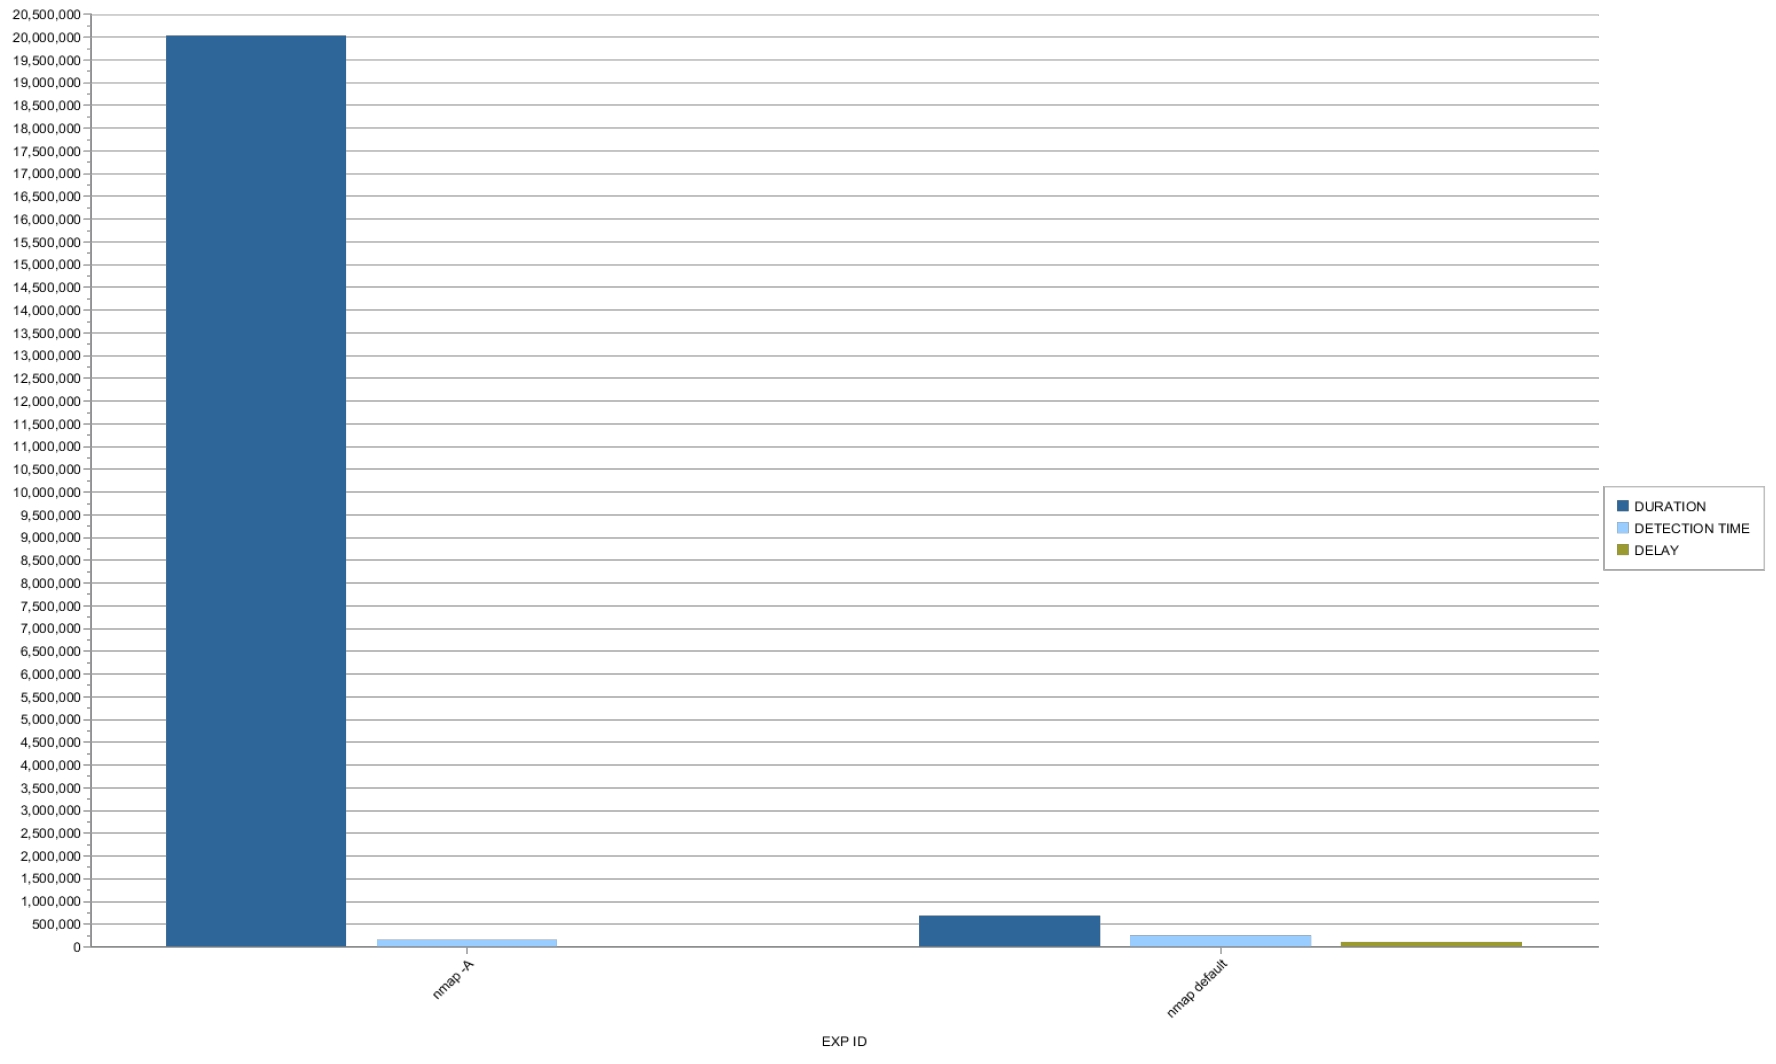
\includegraphics[scale=0.3]{figure/tempi_nmap_A.jpg}\\

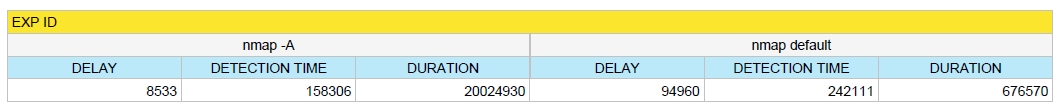
\includegraphics[scale=0.5]{figure/tabella_nmap_A.jpg}

\subsection{Nmap, --osscan-guess vs Default}
Come descritto dal manuale di nmap, utilizzando l'opzione --osscan-guess si esegue un attacco più aggressivo, destinato, quindi, a terminare prima. Snort, come si può vedere dai risultati mostrati dai grafici, riesce a rilevarlo in un tempo più breve rispetto ad una scansione più cauta che quindi passa in principio più inosservata.\\

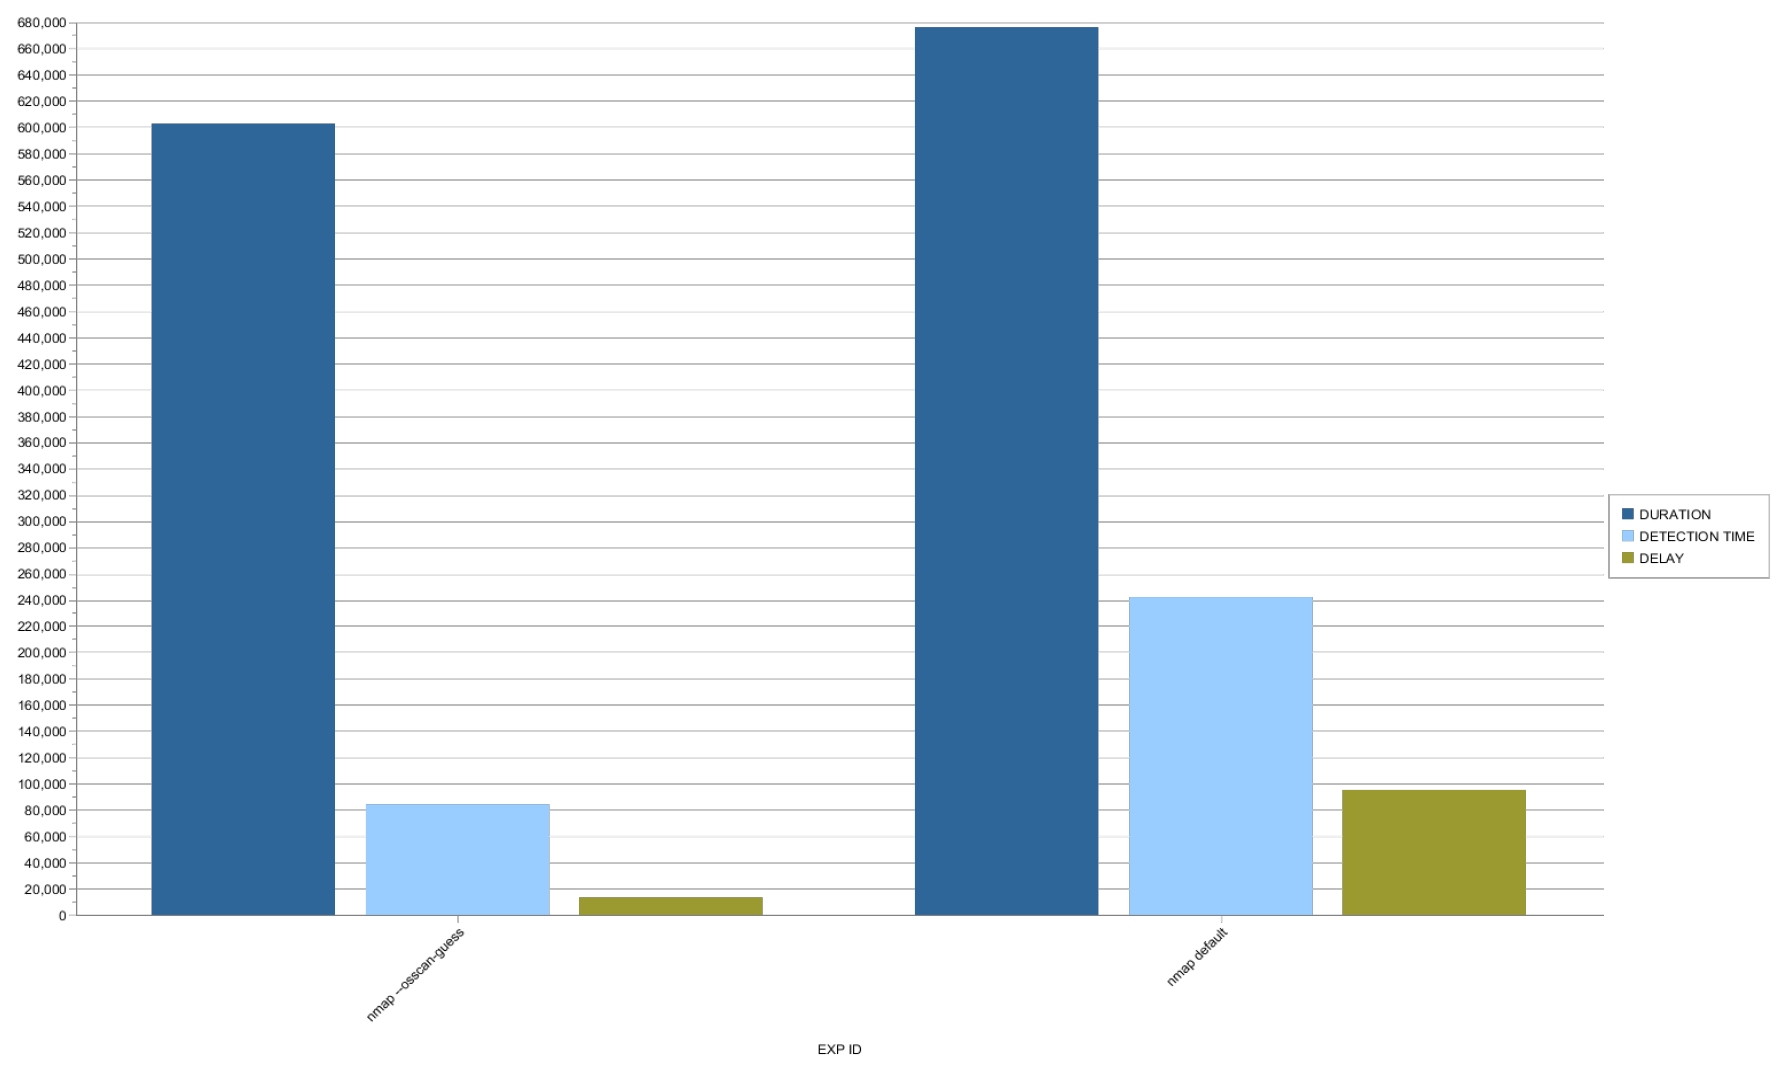
\includegraphics[scale=0.3]{figure/tempi_nmap_osscan.jpg}\\

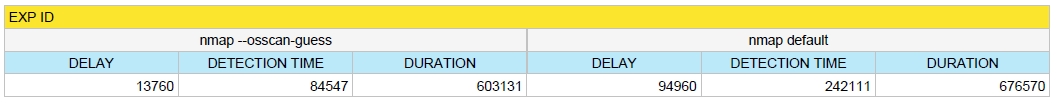
\includegraphics[scale=0.5]{figure/tabella_nmap_osscan.jpg}

\subsection{Nmap, --min-rate 100/300/500 vs Default}
Dalla comparazione dei grafici ottenuti dall'utilizzo di diversi valori (100, 300 e 500 pacchetti/secondo) per l'opzione \textit{--min-rate} del comando nmap possiamo dedurre, intuitivamente, che forzare l'attacco ad inviare più pacchetti al secondo rende l'attacco più veloce e più facilmente rilevabile, dal momento che il numero/tipo di pacchetti necessari a Snort per rilevare l'attacco arrivano con frequenza maggiore. Comparando, inoltre, questi risultati con la versione standard (senza opzioni) di nmap, possiamo ipotizzare che quest'ultima invii i pacchetti necessari ad un rate maggiore di 500 pacchetti/secondo (si vede facilmente seguendo la curva dei tempi di rilevamento). Infine, comparando anche la durata totale dell'attacco, possiamo dedurre che la versione default di nmap esegue più operazioni (o operazioni più complesse) rispetto alla versione che utilizza l'opzione \textit{--min-rate}.\\

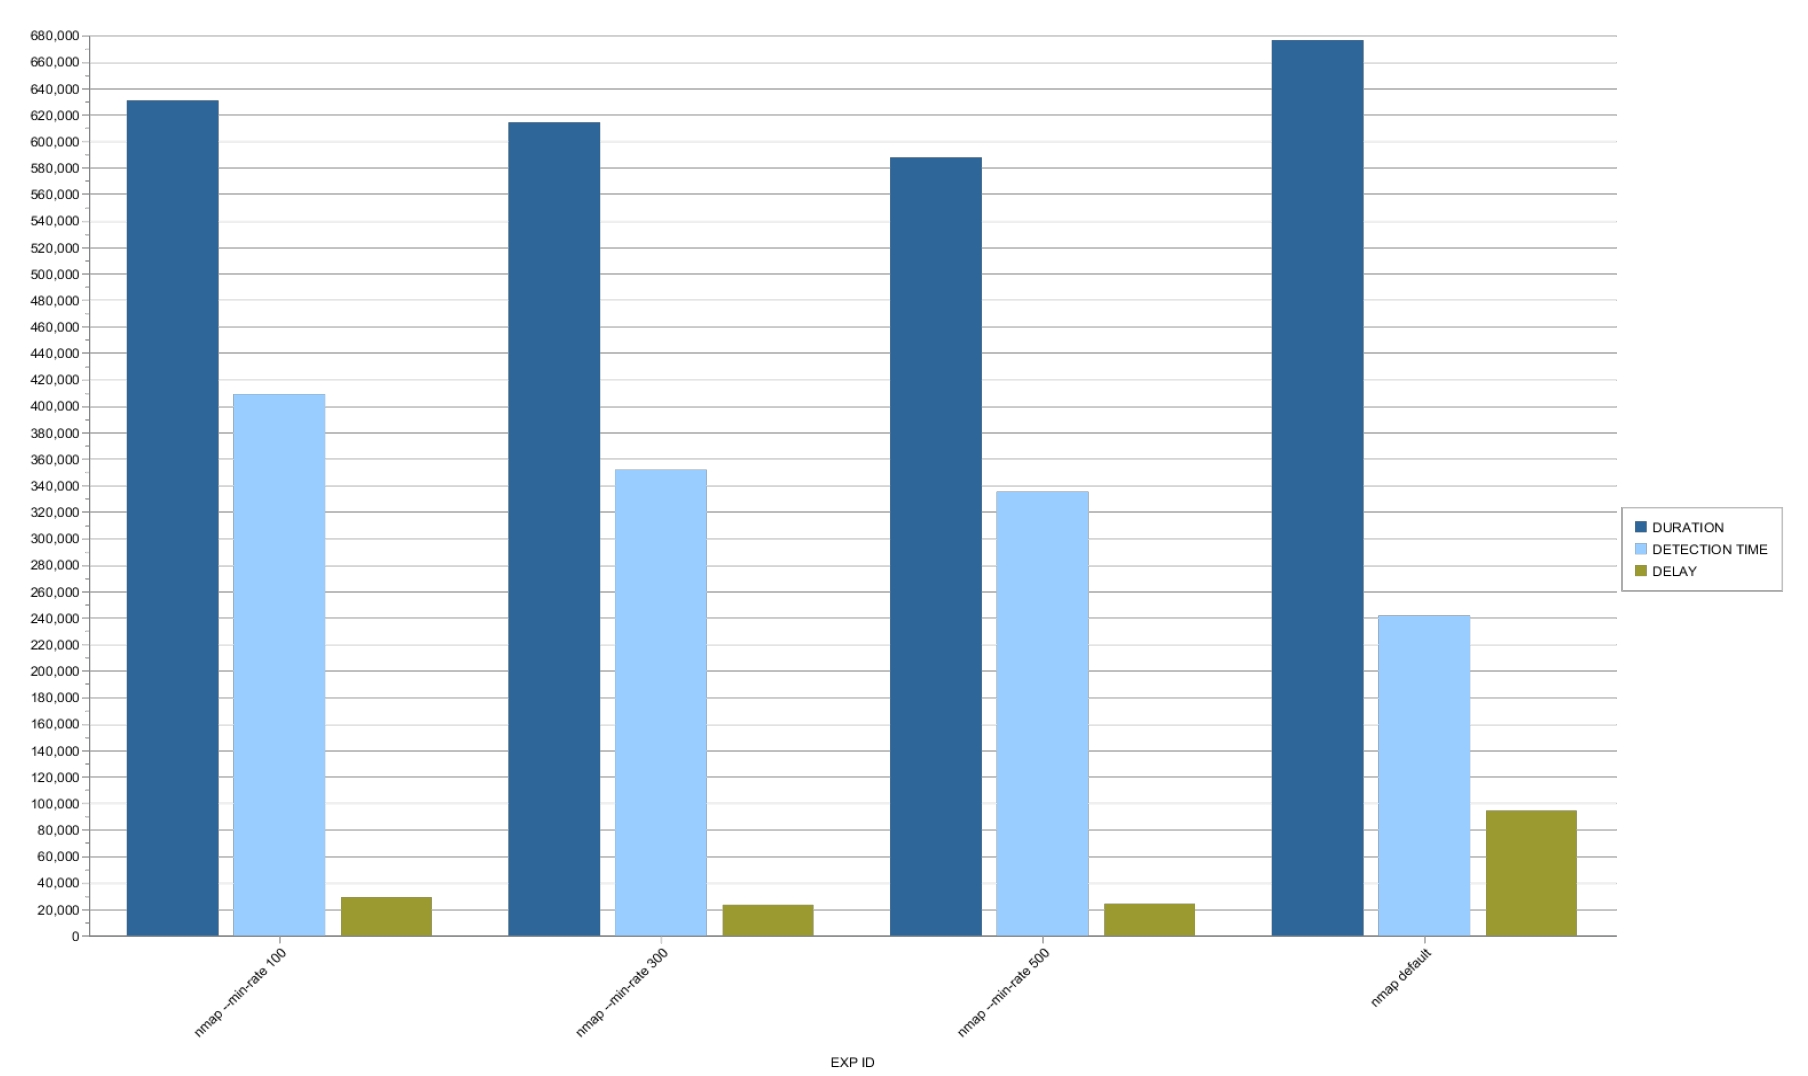
\includegraphics[scale=0.3]{figure/tempi_nmap_minrate.jpg}\\

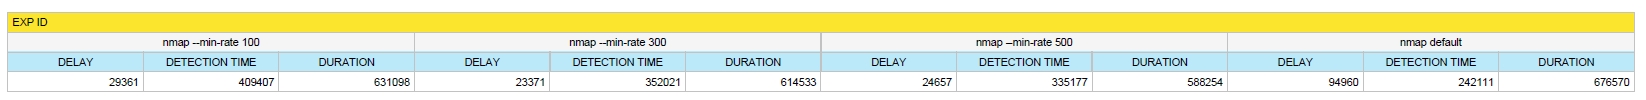
\includegraphics[scale=0.3]{figure/tabella_nmap_minrate.jpg}

\subsection{Nmap, -T 2/3/4/5 vs Default}
Notiamo innanzitutto come le tempistiche di durata e di rilevamento per l'attacco "educato" di nmap (per comodità visualizzato in un grafico a parte) siano fuori scala rispetto a tutti gli altri timing templates. Questo tipo di attacco è infatti stato progettato per agire lentamente, cercando di ridurre al minimo ogni possibile rilevamento da parte di un ipotetico IDS. Per quanto riguarda gli altri templates, possiamo dedurre che l'attacco "aggressivo" (\textit{-T4}) è probabilmente il miglior punto d'incontro tra velocità d'attacco e furtività, permettendo una rapida scansione in grado di aggirare per breve tempo un generico IDS.\\

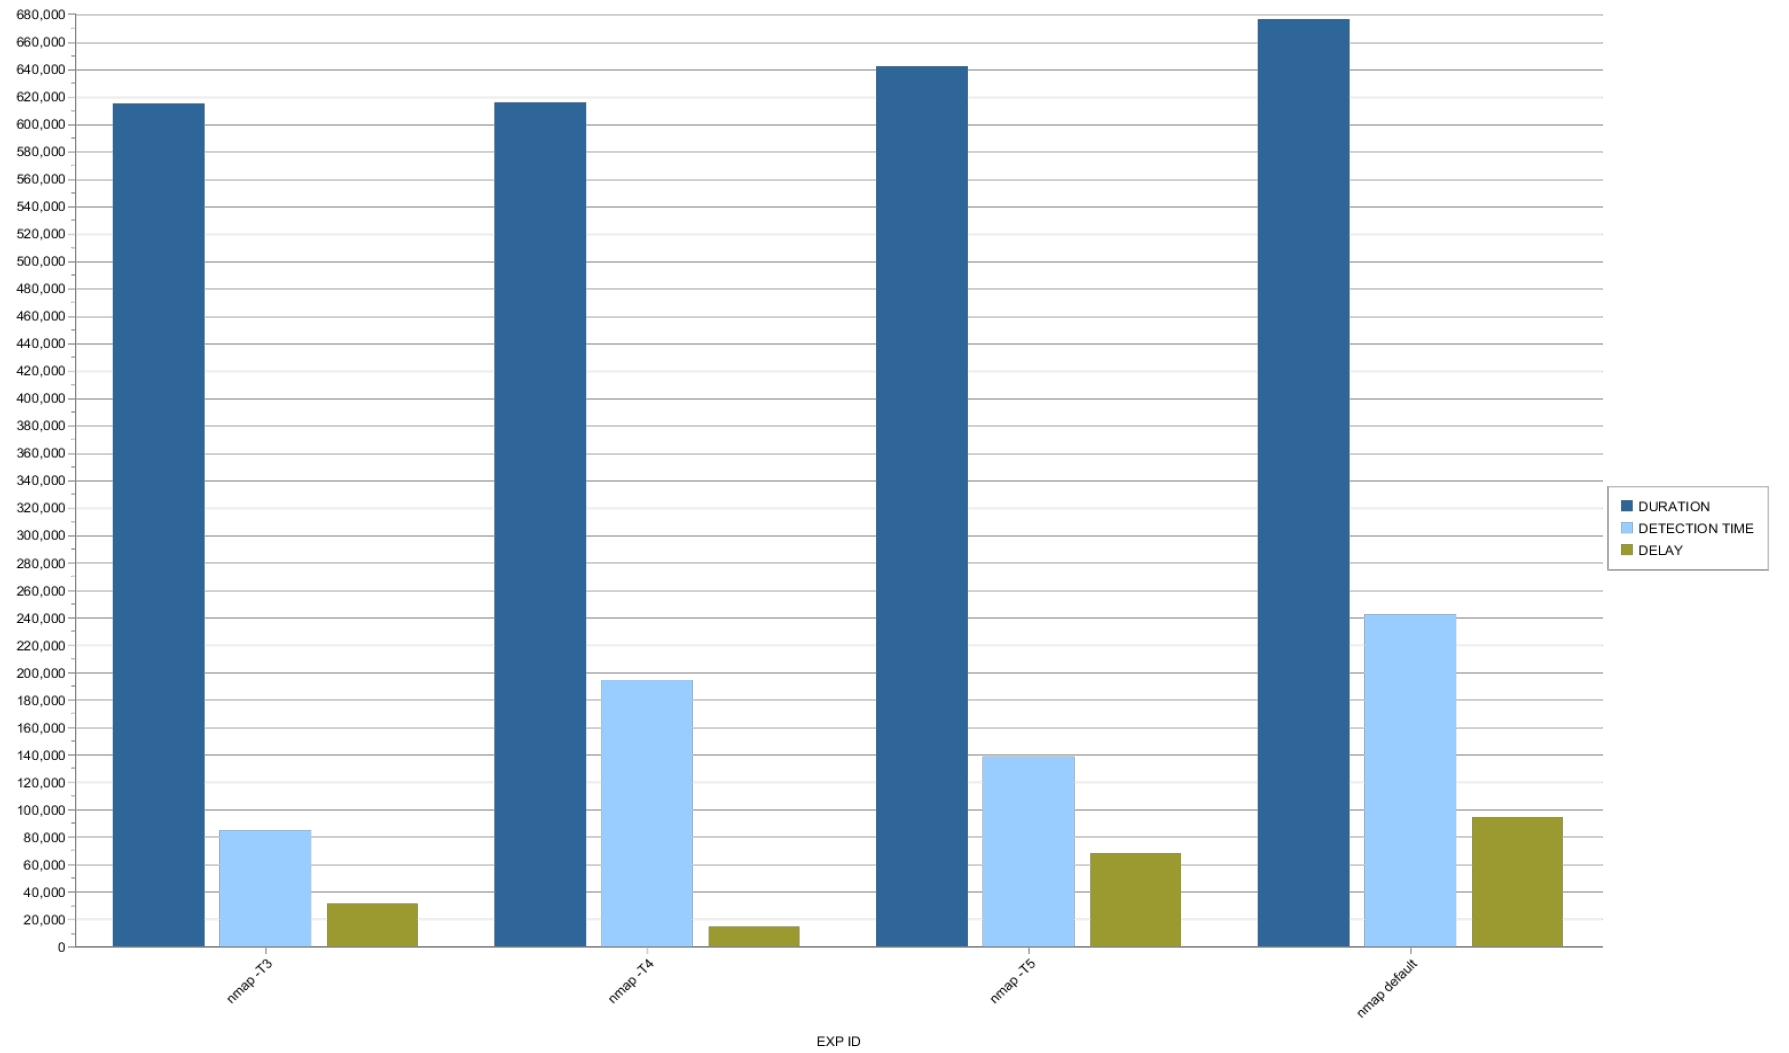
\includegraphics[scale=0.3]{figure/tempi_nmap_T.jpg}\\

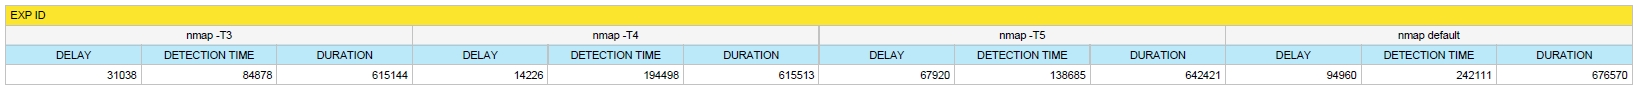
\includegraphics[scale=0.3]{figure/tabella_nmap_T.jpg}\\

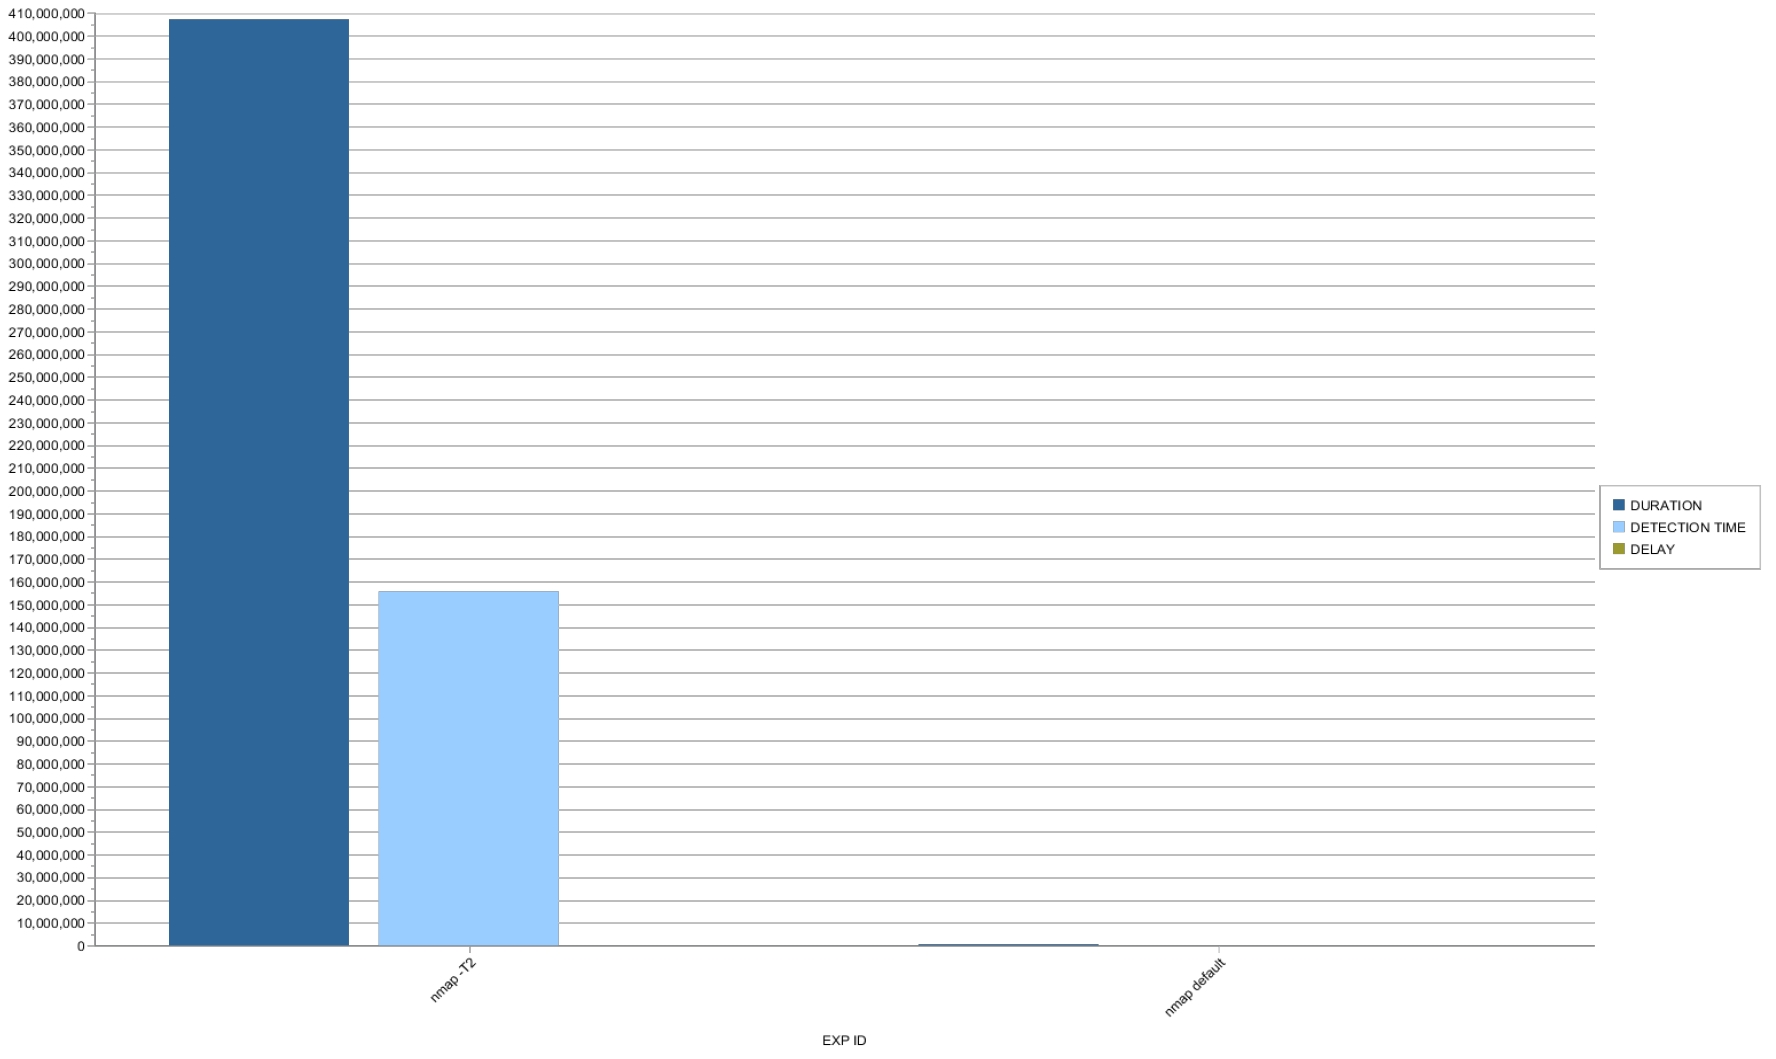
\includegraphics[scale=0.3]{figure/tempi_nmap_T2.jpg}\\
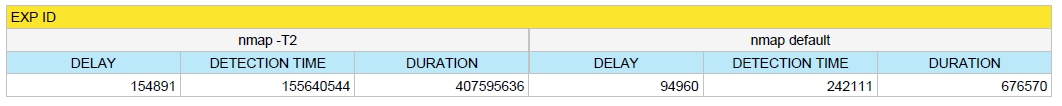
\includegraphics[scale=0.4]{figure/tabella_nmap_T2.jpg}

\subsection{Nmap, --version-all/light vs Default}
Osservando il grafico seguente, ed in particolare le colonne relative al tempo di detection dell'attacco, si vede subito come la versione leggera (\textit{--version-light}) sia più velocemente riconoscibile da un IDS come Snort rispetto alla sua controparte esaustiva (\textit{--version-all}). Confrontando questi risultati con la versione standard di nmap possiamo inoltre supporre che quest'ultima sia formata da un tradeoff delle versioni light e all, in quando il suo tempo di rilevazione si trova più o meno tra i due sopra citati.\\

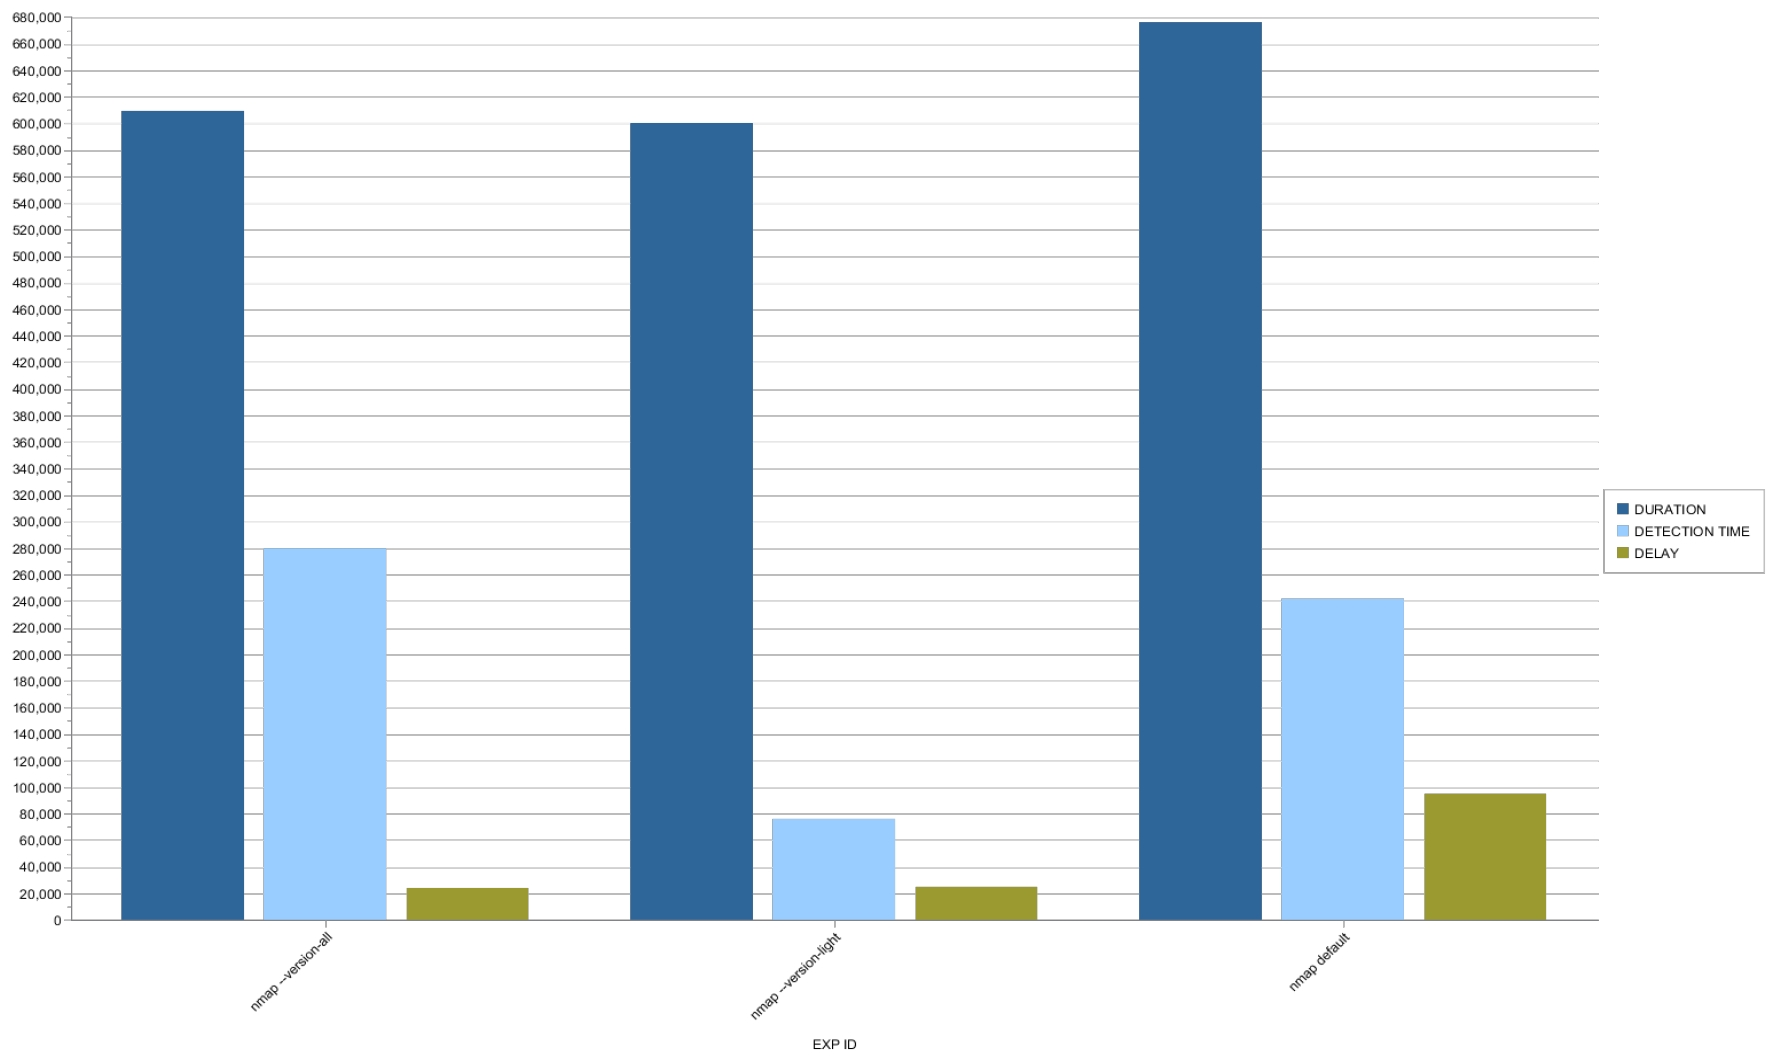
\includegraphics[scale=0.3]{figure/tempi_nmap_all-light.jpg}\\

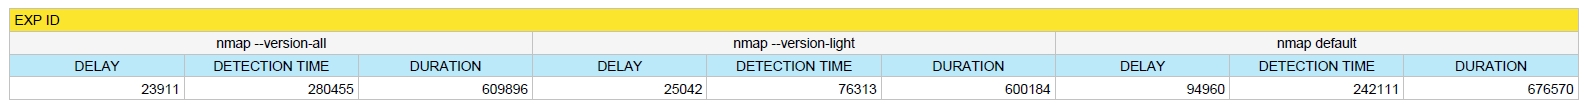
\includegraphics[scale=0.3]{figure/tabella_nmap_all-light.jpg}

	\section{Ping}
Per quanto riguarda l'utilizzo del comando \textit{ping} l'opzione utilizzata è la \textit{-i} con i valori 0.001/0.1/0.3/0.5.\\
Come già accennato in precedenza, Snort rileva immediatamente un qualsiasi attacco basato su pacchetti ICMP, come ad esempio gli attacchi che utilizzano il comando ping (ping of death, denial of service, ...). Questo si vede facilmente dai grafici che mostrano come in tutti i casi il tempo di rilevamento da parte di Snort di un attacco ping sia immediato. Per quanto riguarda invece la durata complessiva dell'attacco si ha che, come ci si può aspettare, a parità di pacchetti inviati (100, in questi esperimenti) la durata dell'attacco aumenta al diminuire del rate di invio: inviando ad un rate di 0.001 pacchetti/secondo l'attacco termina in meno di mezzo secondo, mentre inviando ad una frequenza di 0.5 pacchetti/secondo la durata aumenta fino a quasi 50 secondi complessivi\\
Inoltre dall'analisi dei log è possibile osservare che per un rate di invio pare a 0.5 pacchetti/secondo non viene generato alcun alert del tipo \textit{``TOO MUCH PING''}, verificando che l'introduzione della nostra regola permette di stabilire una soglia oltre la quale si può ritenere dannosa la sottomissione di ping troppo frequenti.

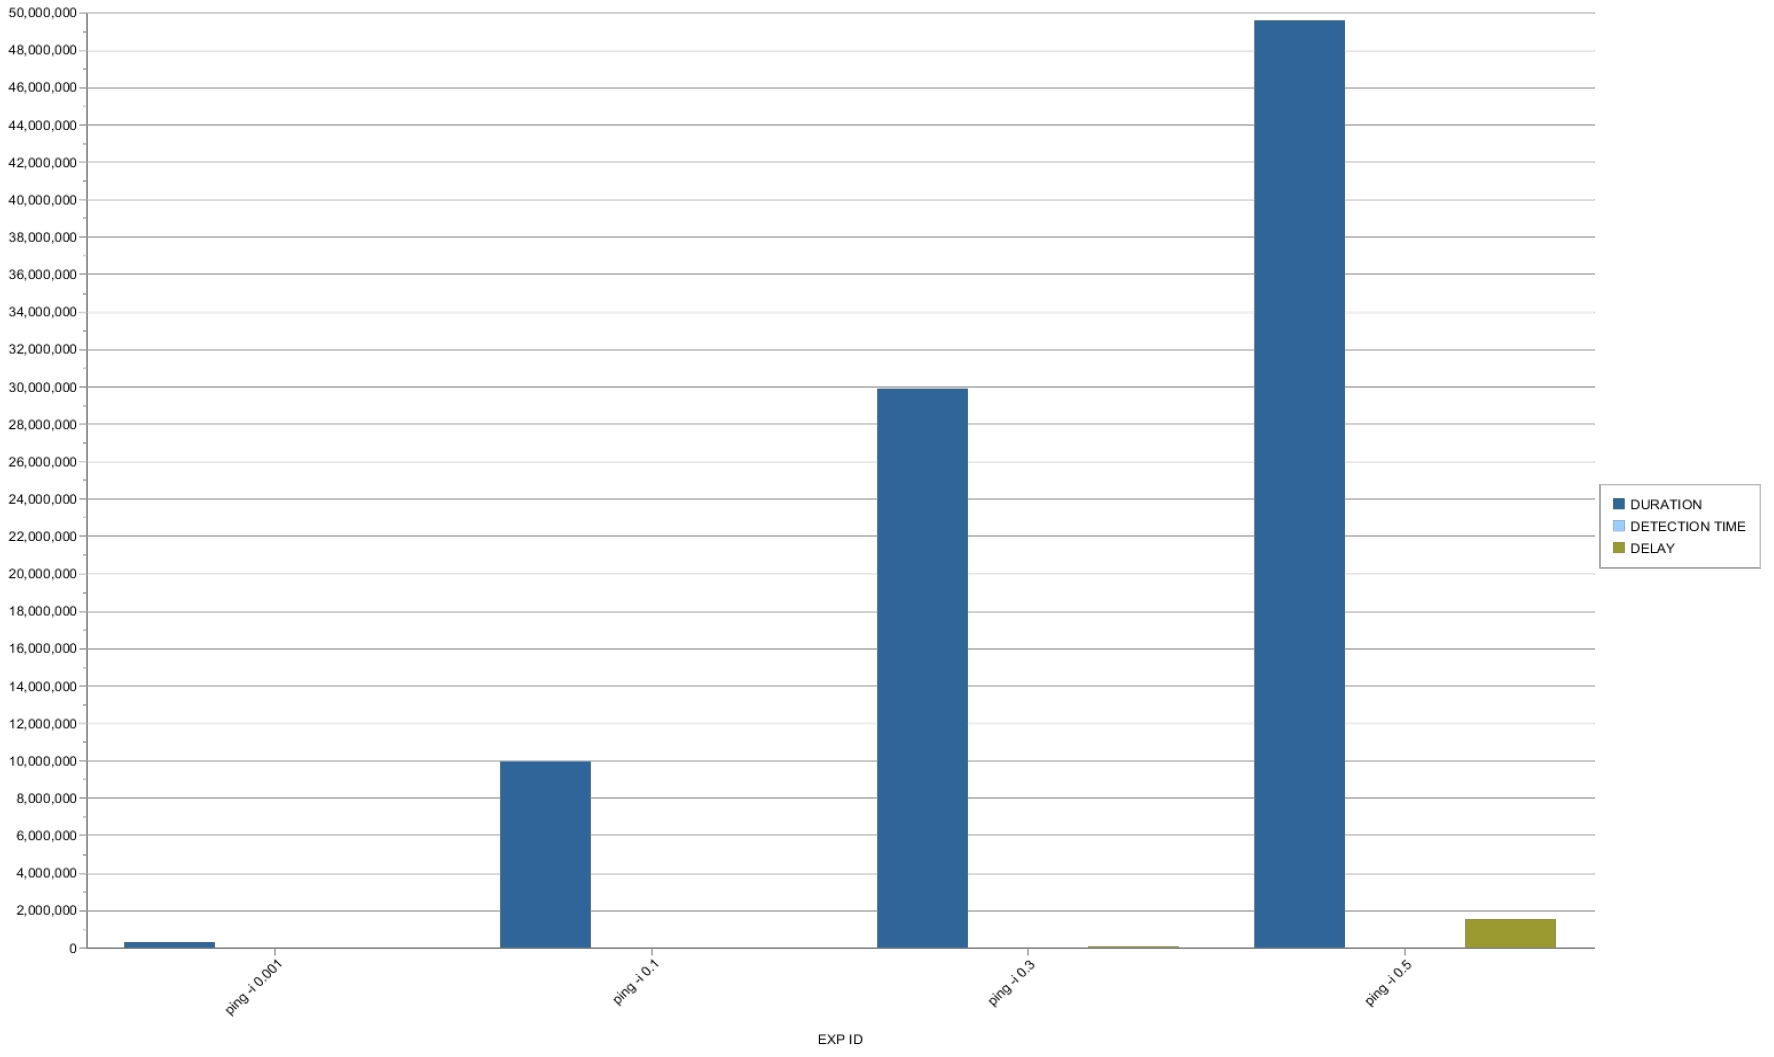
\includegraphics[scale=0.3]{figure/tempi_ping.jpg}\\

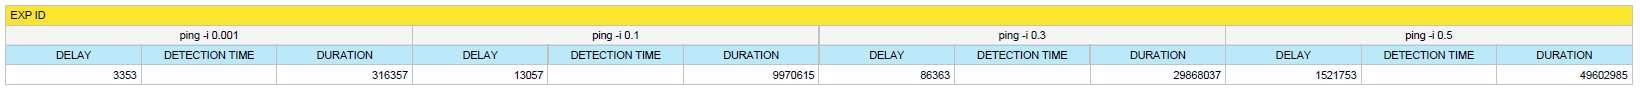
\includegraphics[scale=0.3]{figure/tabella_ping.jpg}



	\section{Metasploit}
Metasploit è stato utilizzato come port scan nella sua versione di default e successivamente abilitando l'opzione \textit{Scan SNMP}.\\
Dai grafici si nota come la versione standard dell'attacco di Metasploit sia più corta rispetto alla versione completa, probabilmente a causa delle operazioni in più che quest'ultima compie. Inoltre possiamo vedere che il tempo di detection dell'attacco standard è più alto rispetto alla versione avanzata, che invece viene rilevata subito da Snort, forse a causa delle tecniche di intrusione più aggressive introdotte da quest'ultima.\\

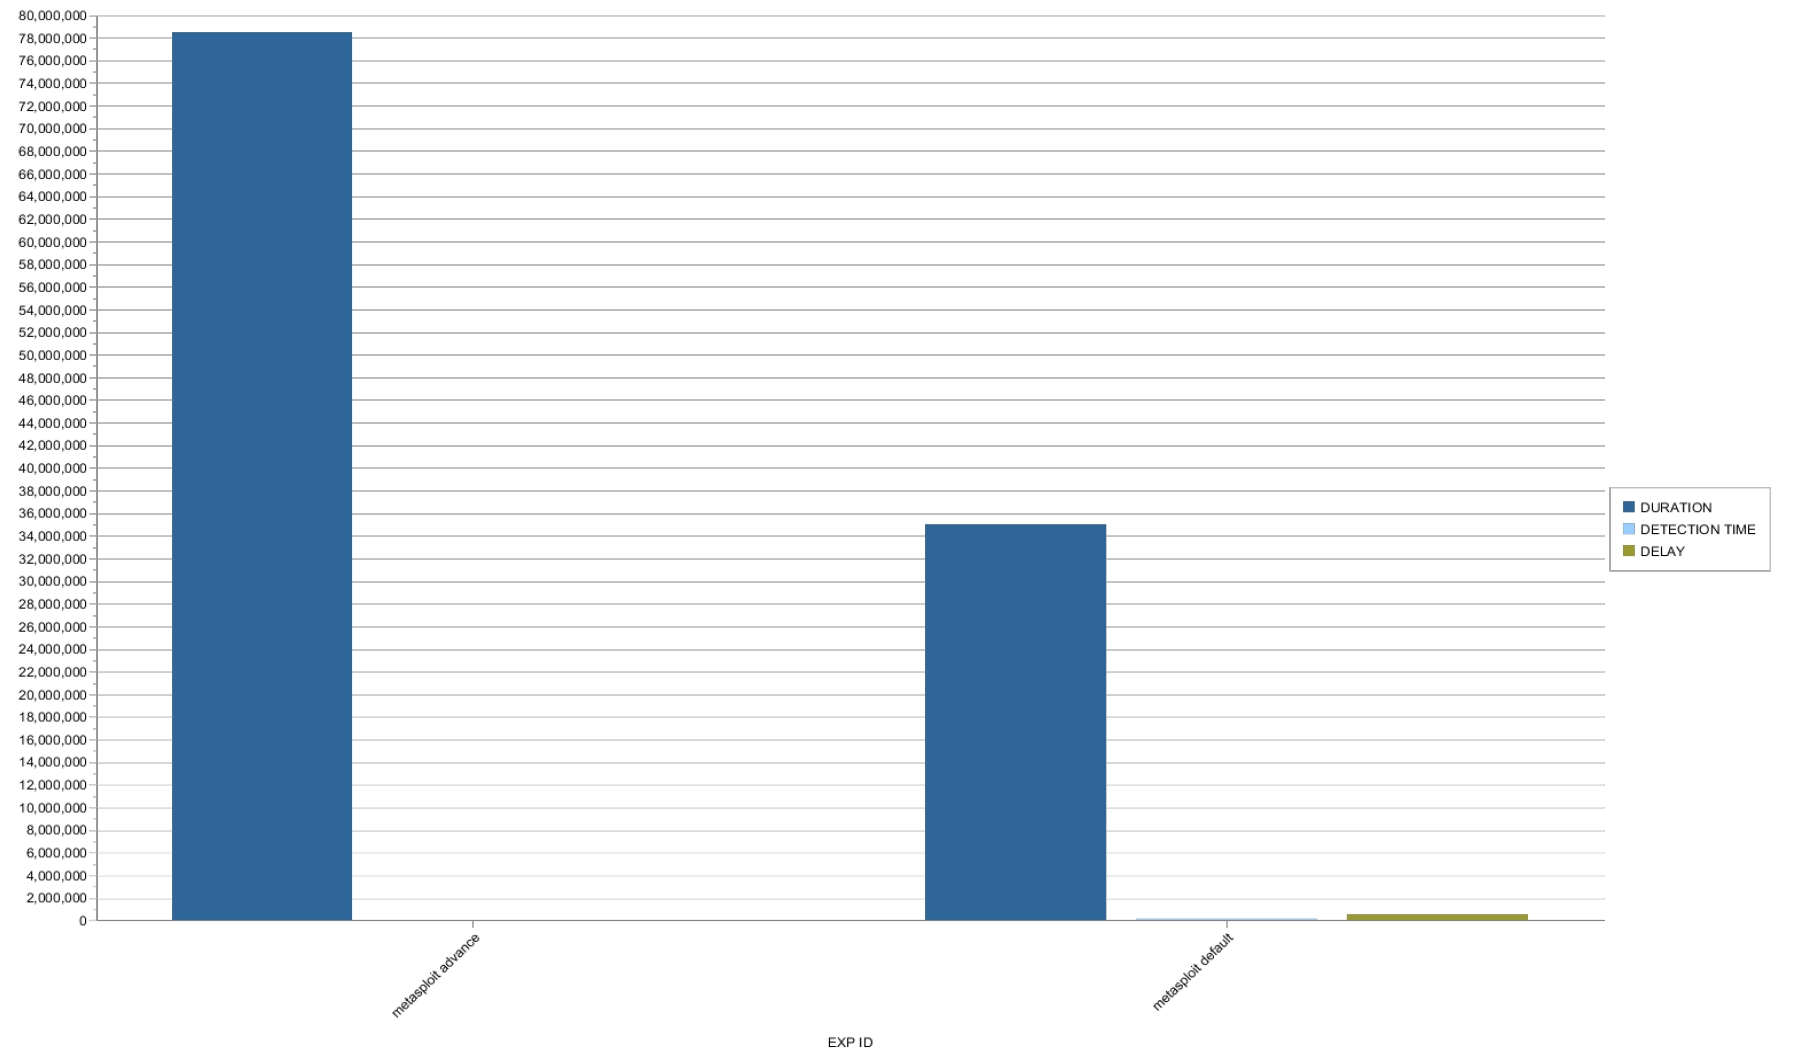
\includegraphics[scale=0.3]{figure/grafico_metasploit.jpg}\\

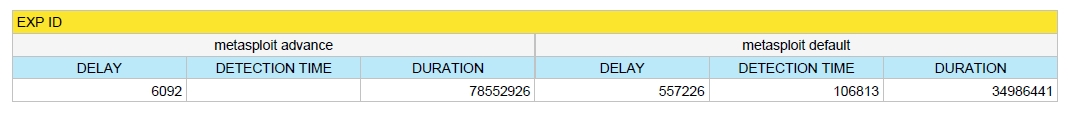
\includegraphics[scale=0.3]{figure/tempi_metasploit.jpg}


	\section{Traceroute}

\subsection{Traceroute, -N 20/30/40 vs Default}
Osservando i valori della detection si vede come questi siano esattamente identici (68 microsecondi) per i tre esperimenti con l'opzione -N, mentre sia leggermente più bassa (42 microsecondi) per quanto riguarda l'attacco traceroute di default. Rispetto alla durata dell'attacco, come ci si aspetta questa aumenta all'aumentare del numero di pacchetti-sonda inviati dal comando, mentre rimane circa a metà strada tra -N 30 e -N 40 per quanto riguarda la versione standard di traceroute. Quindi, dal momento che il manuale afferma che il valore di default per i pacchetti-sonda è 16, dai valori di durata della versione standard possiamo supporre che quest'ultima esegua operazioni in più, o più complesse, rispetto al comando che utilizza l'opzione -N.\\

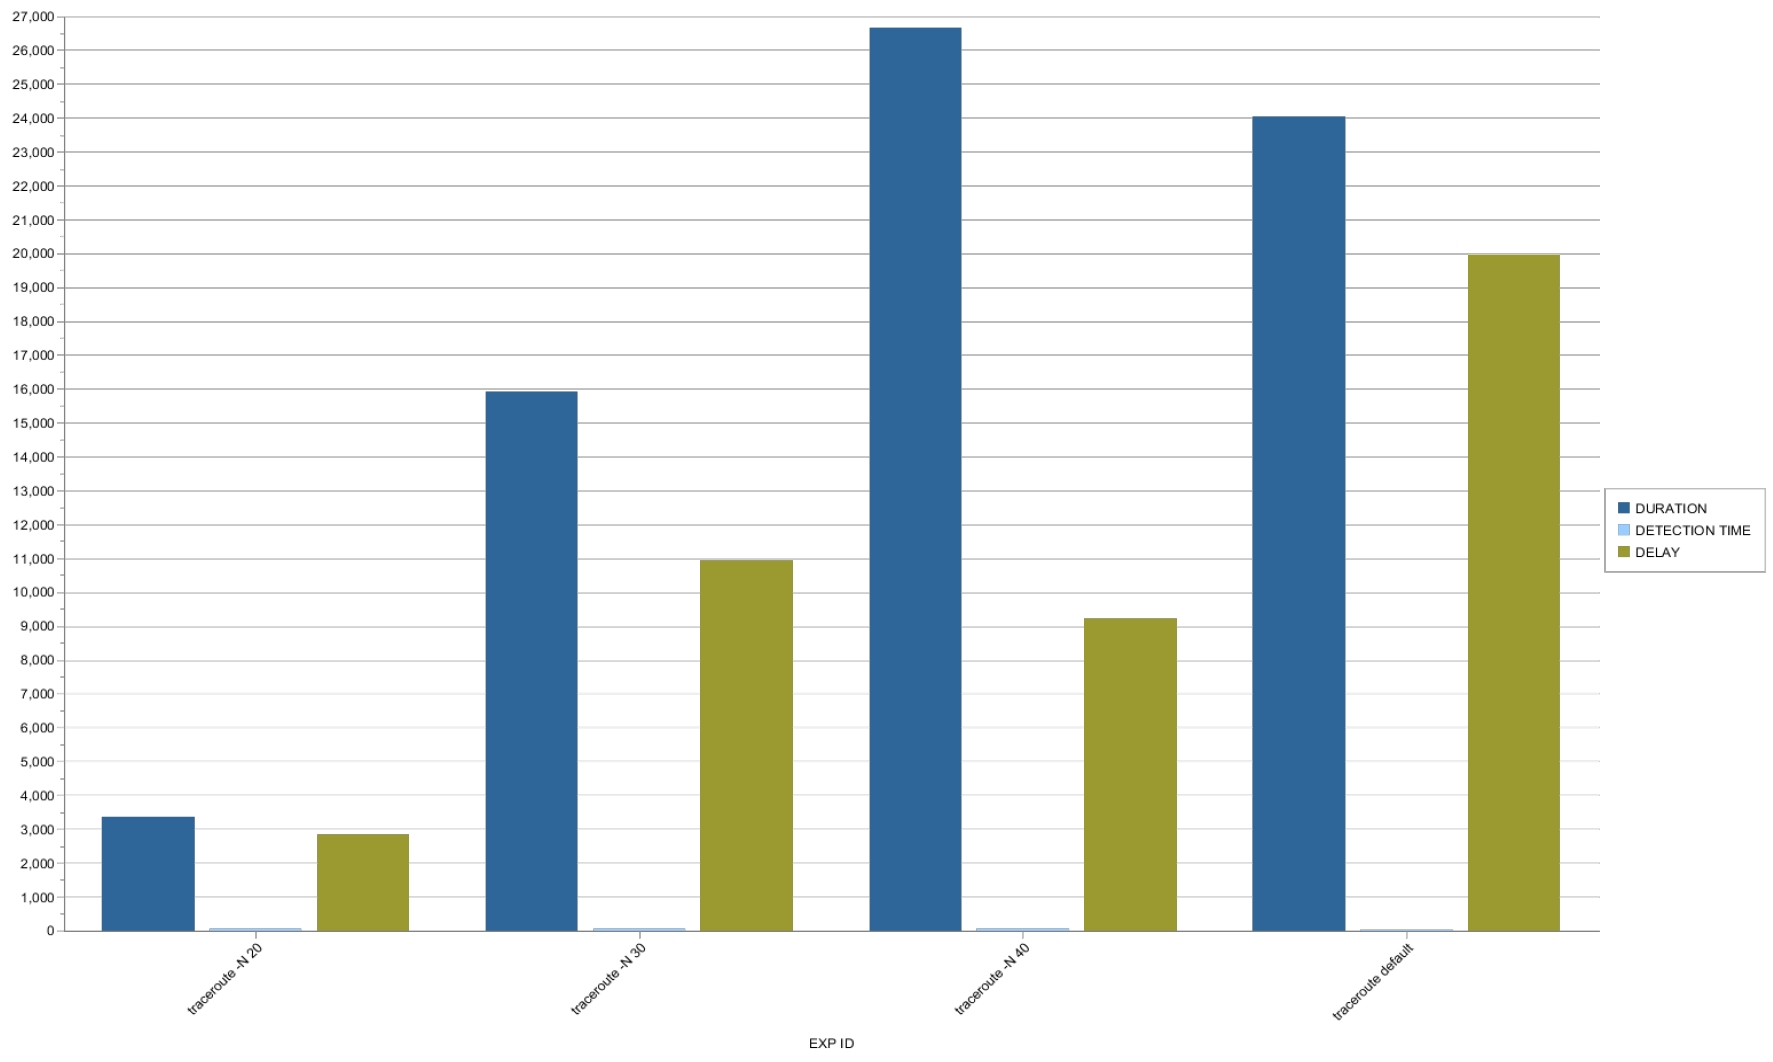
\includegraphics[scale=0.3]{figure/tempi_traceroute_N.jpg}\\

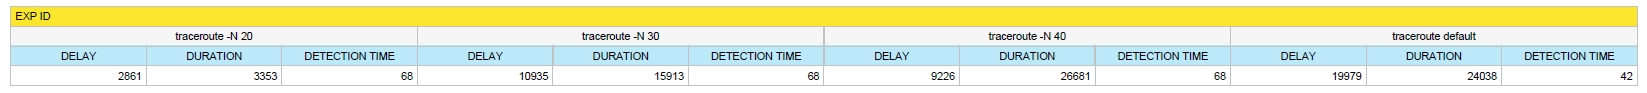
\includegraphics[scale=0.3]{figure/tabella_traceroute_N.jpg}

\subsection{Traceroute, -T vs Default}
In questi grafici, per comodità, sono stati omessi i valori di detection in quanto, come già accennato, il comando traceroute con opzione -T non genera alcun alert da parte di Snort. Si è comunque deciso di includere gli altri valori in quanto, dalla parte del sistema attaccato, vengono comunque ricevuti e loggati molti pacchetti che evidenziano, ad esempio, la maggior complessità dell'attacco traceroute -T, che impiega più tempo a terminare la scansione rispetto alla versione standard di traceroute.\\

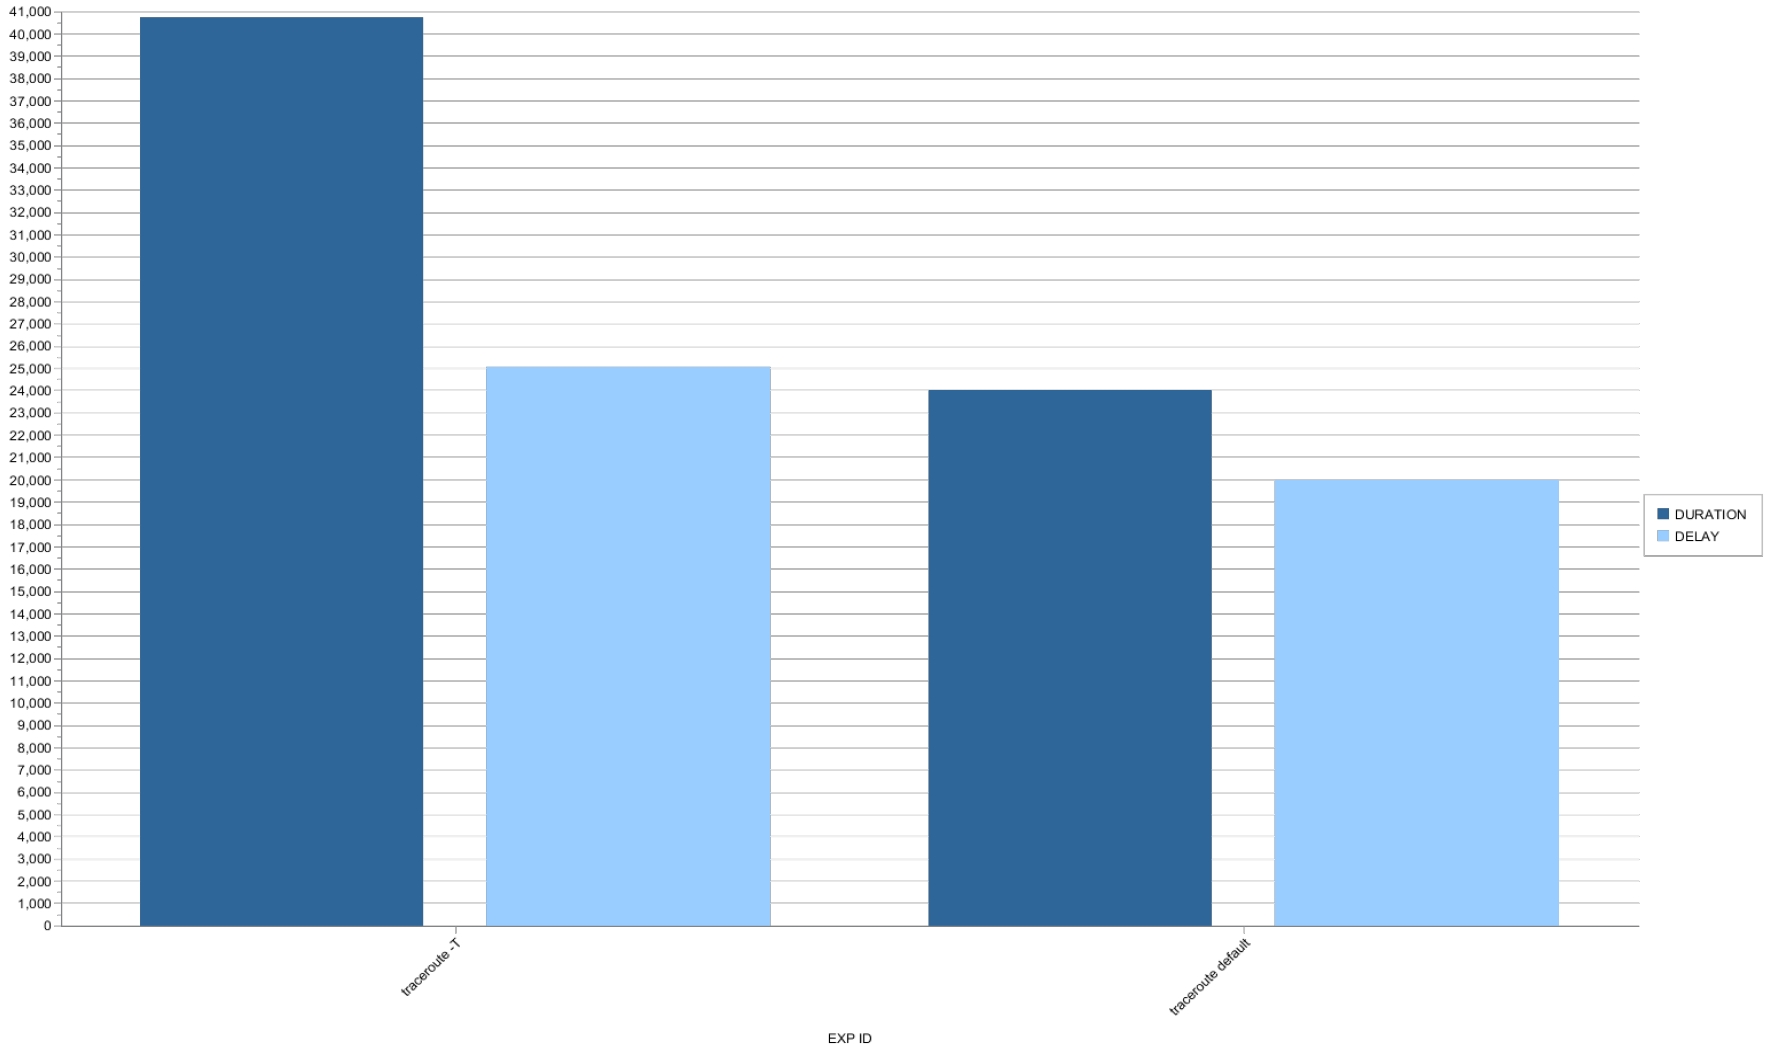
\includegraphics[scale=0.3]{figure/tempi_traceroute_T.jpg}\\

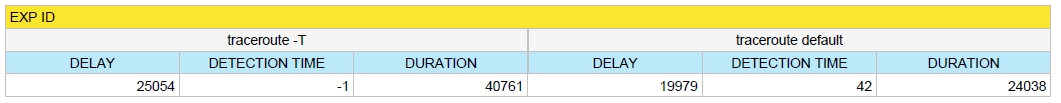
\includegraphics[scale=0.3]{figure/tabella_traceroute_T.jpg}

\subsection{Traceroute -I vs Default}
Come ci potevamo attendere, indicando a traceroute di eseguire un attacco tramite pacchetti ICMP ECHO si avrà che quest'attacco verrà identificato immediatamente (ovvero all'arrivo del primo pacchetto) da parte di Snort sul sistema attaccato. Infatti sappiamo che qualsiasi ping ricevuto da Snort verrà immediatamente loggato come alert. A parte questo, notiamo come (analogamente a quanto visto per l'opzione -T) la durata complessiva dell'attacco sia maggiore includendo l'opzione -I, che probabilmente aggiunge complessità all'attacco base di traceroute.\\

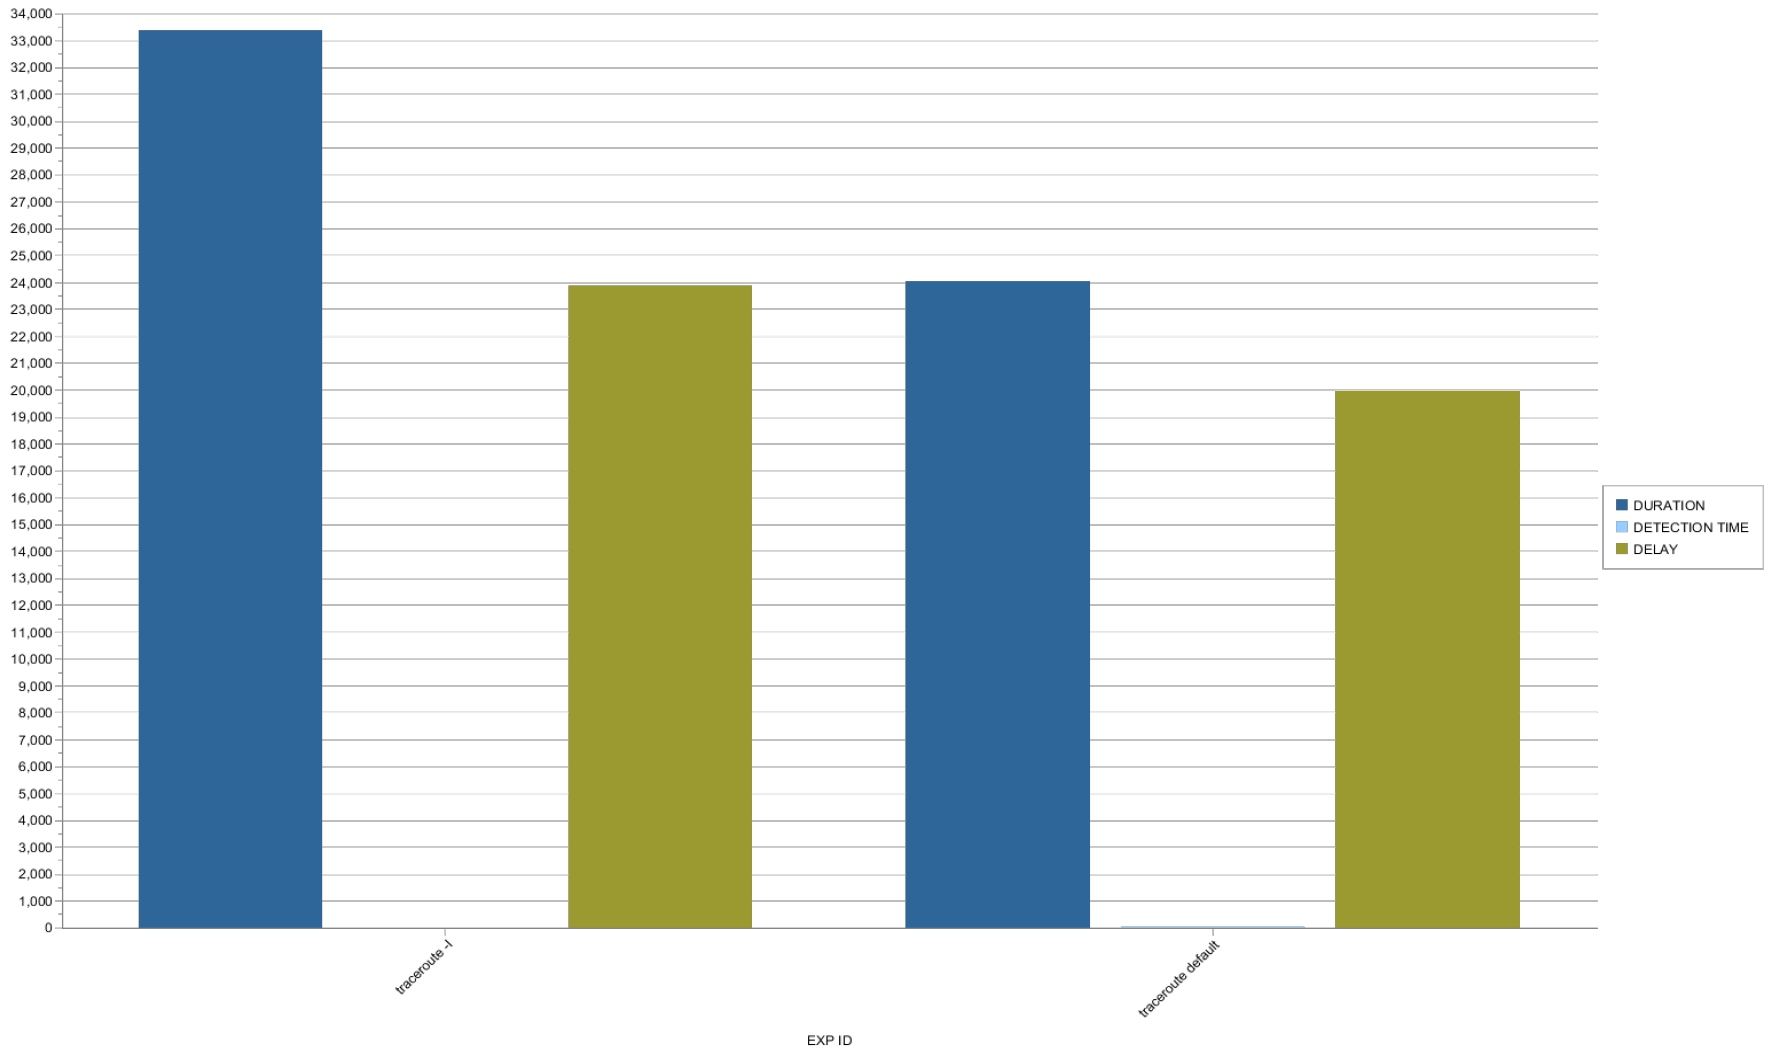
\includegraphics[scale=0.3]{figure/tempi_traceroute_I.jpg}\\

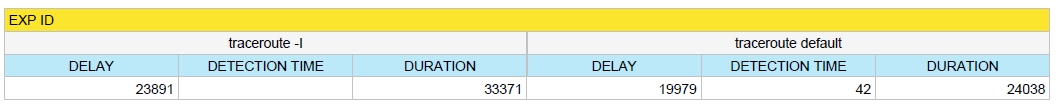
\includegraphics[scale=0.3]{figure/tabella_traceroute_I.jpg}

	\section{Protocolli}

Analizzando le tempistiche di detection per i tre protocolli principali utilizzati in questi esperimenti (ICMP, TCP ed UDP) si nota innanzitutto come i tempi di rilevamento per attacchi basati su ICMP (ad es. ping) sia pressoché nulla, rendendo inefficace un qualsiasi tipo di attacco. Per quanto riguarda invece TCP e UDP notiamo un netto distacco, a favore di TCP, secondo i tempi di detection: è possibile, dato che UDP è un protocollo non affidabile che punta tutto sulla velocità d'invio, che gli attacchi basati su UDP siano progettati in modo da agire velocemente, velocizzando quindi anche il processo di rilevazione da parte degli IDS in ascolto, mentre un attacco basato su TCP potrebbe agire più lentamente ed in modo più silenzioso. Un'altra possibile spiegazione è che, dato che il protocollo TCP è affidabile per natura, molte analisi su questi pacchetti vengono già fatte dalla stessa infrastruttura di rete, quindi è possibile che un IDS come Snort decida di dare meno peso (con meno regole o regole meno stringenti) a questo tipo di pacchetti, preferendo invece concentrarsi su pacchetti meno controllati come quelli UDP o ICMP. Osservando invece la durata media degli attacchi raggruppata per protocollo, vediamo come gli attacchi ICMP siano mediamente i più veloci (pensiamo ad attacchi come ping o nmap -I), subito seguiti da attacchi TCP e da attacchi UDP, che evidentemente fanno, in media, più operazioni (o operazioni più complesse) rispetto agli attacchi basati su ICMP o TCP.

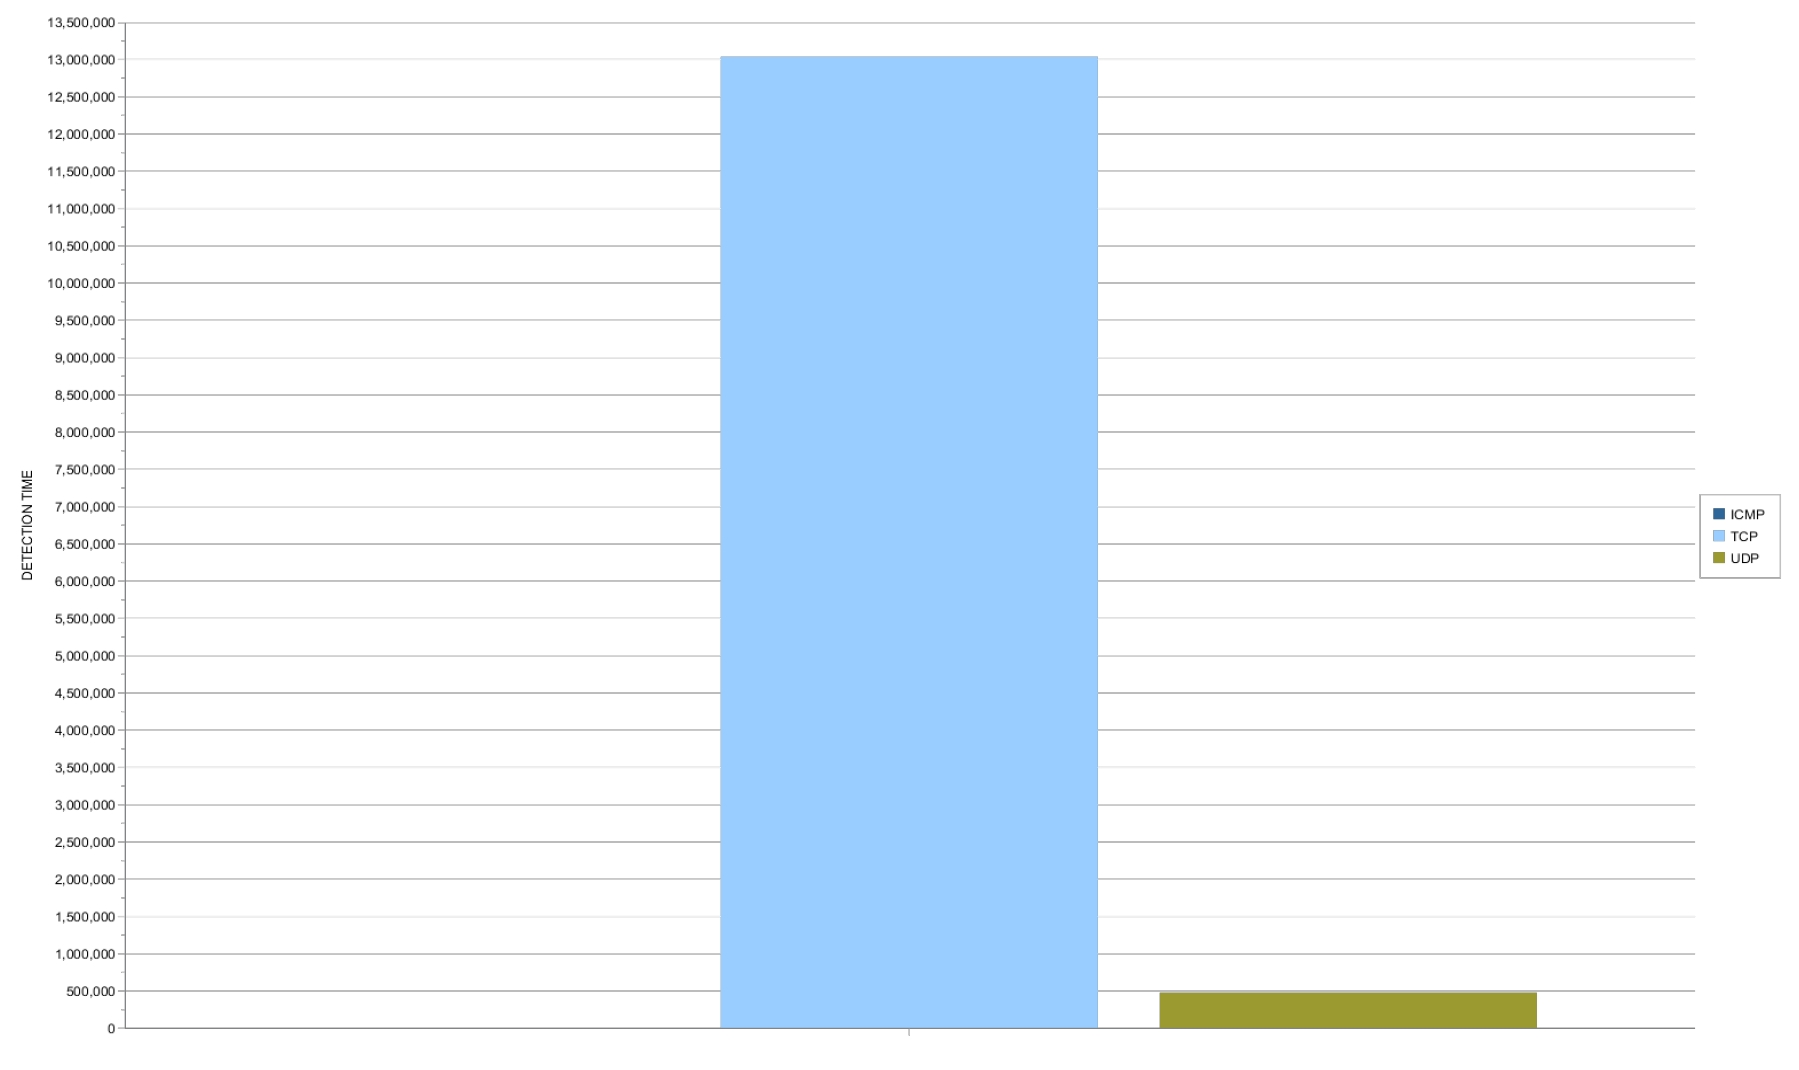
\includegraphics[scale=0.3]{figure/detection_protocol.jpg}\\

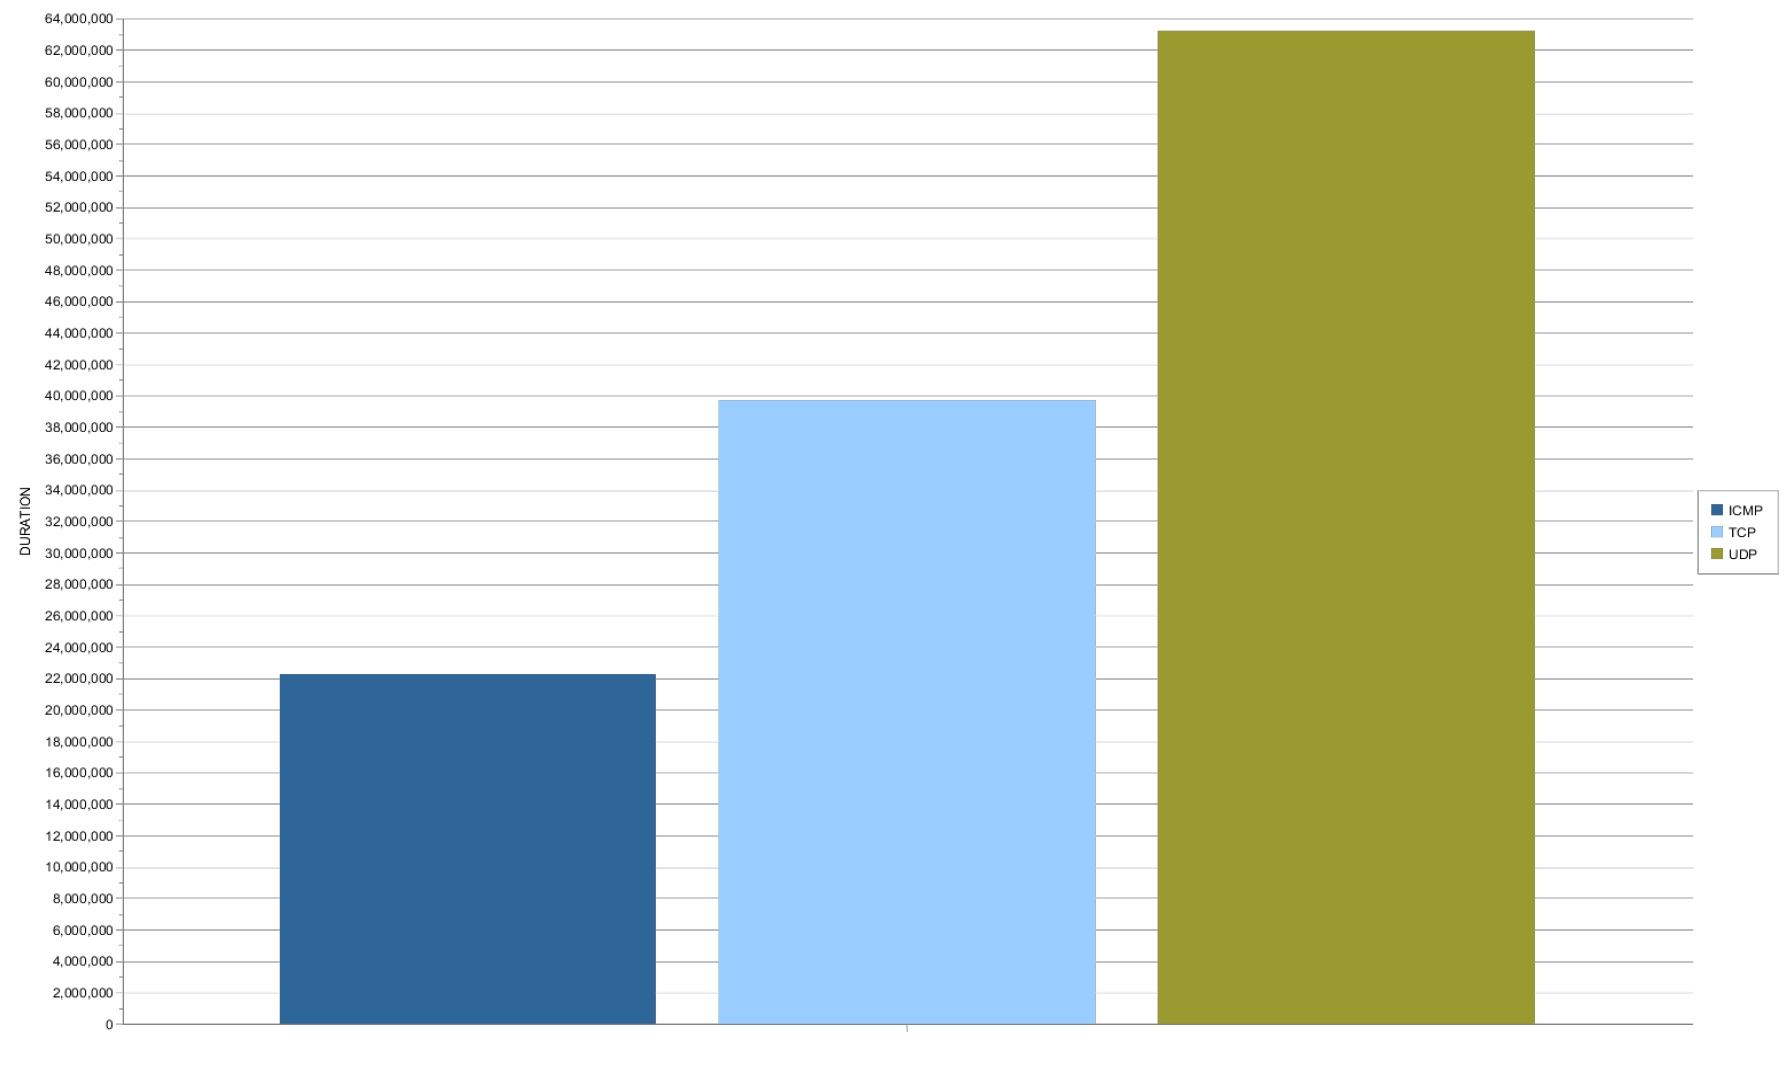
\includegraphics[scale=0.3]{figure/duration_protocol.jpg}\\

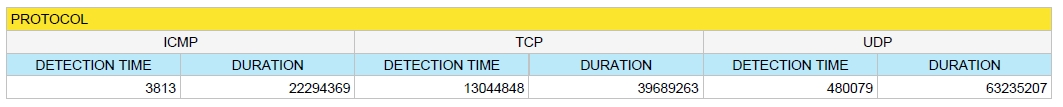
\includegraphics[scale=0.4]{figure/tabella_protocolli.jpg}

	\section{Alert generati}

Esponiamo per una più chiara interpretazione del grafico a seguito di che genere di eventi gli alert vengono generati:

\begin{itemize}

    \item \textbf{ICMP PING undefined code}, questo alert vine generato quando un utente esterno effettua un ping su un server interno usando una richiesta di tipo echo ICMP. Generalmente un attaccante utilizza scansioni di questo tipo per ottenere informazioni sul network o inviare un elevato numero di ping nel tentativo di causare un flood della rete per creare un DoS.

    \item \textbf{ICMP Echo Reply undefined code}, questo alert viene generato quando un host genera una risposta di tipo echo ICMP, (con un codice ICMP non valido o non denito). \'E evidente che questo messaggio è speculare rispetto al precedente: l'host di destinazione invia un messaggio di risposta all'host richiedente indicando quindi di essere alive.

    \item \textbf{SNMP AgentX/tcp request}, questo alert viene generato quando si tenta di attaccare un dispositivo utilizzando SNMP v1. L'impatto varia in base all'implementazione, da un tentativo di Denial of Service (DoS) all'esecuzione di codice. SNMP (Simple Network Management Protocol) è un protocollo largamente adottato per reti IP, utile ai ni di manutenzione e monitoring.

    \item \textbf{SNMP request tcp}, questo alert viene generato quando si invia una richiesta per determinare se un dispositivo stia usando l'SNMP; l'attaccante invia un pacchetto (solitamente diretto alla porta tcp o udp 161), e se ciò avviene con successo viene generata una risposta, in base alla quale potrà scegliere di inviare eventuali ulteriori attacchi all'SNMP daemon.

    \item \textbf{SHELLCODE x86 inc ebx NOOP}, questo alert viene generato quando è probabile sia stato effettuato un tentativo di eseguire del codice su di un host nella rete protette proveniente da una sorgente esterna a tale rete.

    \item \textbf{SCAN nmap XMAS}, questo alert viene generato quando è stata individuata una scansione da parte della piattaforma XMAS di Nmap.Generalmente avviene quando un attaccante effettua una scansione con Nmap al fine di determinare quali siano le porte aperte, esattamente ciò che abbiamo effettuato. Ciò significa che SNORT ha individuato la nostra scansione con Nmap.

    \item \textbf{ICMP PING}, questo alert viene generato quando viene effettuata una richiesta ICMP echo di tipo generico per determinare se l'host è attivo. Analogo all'ICMP PING undefined code.
        
    \item \textbf{ICMP Echo Reply}, analogo all'ICMP PING Echo Reply undefined code.
    
    \item \textbf{ICMP Destination Unreachable Port Unreachable}, questo alert può indicare che che qualcuno ha tentato di connettersi ad una porta o ad un sistema non disponibile e che probabilmente la sorgente di un determinato pacchetto sta effettuando una scansione o un'altra attività maligna.
        
    \item \textbf{ICMP PING *NIX}, questo alert indica che è stato effettuato un ping originato da un host su cui è in esecuzione Unix.
        
    \item \textbf{SNMP public access udp}, questo alert viene generato quando si effettua una connessione di tipo SNMP tramite UDP utilizzando la community 'public'; molte implementazioni di SNMP sono preconfigurate con communities 'public' e 'private' e se non vengono disabilitate un attaccante può tentare di ottenere informazioni sul dispositivo.
        
    \item \textbf{SNMP request udp},è un alert analogo all'SNMP request tcp,generato quando si invia una richiesta per determinare se un dispositivo stia usando l'SNMP; in questo caso la porta sulla quale l'attaccante invia un pacchetto è di tipo udp.
        
    \item \textbf{MS-SQL ping attempt}, questo alert viene generato quando si identifica un tentativo di SQL ping nel traffico di rete. SNORT segnala che può essere stato utilizzato Nessus per accertarsi dell'esistenza di un database SQL sull'host e può preludere ad un attacco verso tale servizio o indicare che altri tool siano in uso per determinare lo stato dei server SQL.
        
    \item \textbf{POLICY PCAnywhere server response}, questo alert viene generato quando il traffico di rete indica l'utilizzo di un'applicazione o di un servizio potenzialmente in grado di violare una politica di corporate security. Una violazione della politica di corporate security può manifestare un serio rischio per le attività della compagnia.
        
    \item \textbf{RPC portmap listing UDP 111}, il servizio di mappatura delle porte registra tutti i servizi RPC (Remote Procedure Call) sugli host di tipo UNIX. Quando un evento generato quando è possibile che sia stato effettuato un tentativo di scoprire quali servizi RPC siano offerti e su quali porte siano in ascolto.
        
    \item \textbf{DNS named version attempt}, questo alert viene generato quando viene effettuato un tentativo di scoprire la versione di BIND (Berkeley Internet Name Domain, il più usato specialmente su sistemi Unix) specifica che il server DNS sta eseguendo. Così facendo un potenziale attaccante può scoprire quali server siano potenzialmente vulnerabili a degli exploit associati ad una versione di BIND.
        
    \item \textbf{ICMP traceroute}, questo alert viene generato quando è probabile sia stato identificato Windows traceroute, comando generalmente utilizzato da un attaccante che voglia determinare gli host ed i router attivi su una rete in preparazione di un attacco.
        
    \item \textbf{SNMP missing community string attempt}, questo alert viene generato quando le comunicazioni SNMP non contengono un nome di community. Un nome di community SNMP è il processo di autenticazione che un host, che esegue SNMP, utilizza per concedere l'accesso. Fornendo una community vuota e un attaccante può tentare di ottenere l'accesso a funzionalità SNMP per un dispositivo che non è correttamente ben configurato.
        
    \item \textbf{ICMP PING BSDtype}, questo alert indica che è stata inviata dalla rete una richiesta di ping Questo genere di richieste solitamente vengono utilizzate per determinare se un host è "reponsive", ma sono anche  utilizzabili per mappare la rete.
    
    \item \textbf{TOO MUCH PING}, questo alert viene generato ogni qualvolta che il numero di ping sottomessi al secondo sono più di 10. Permette di rilevare una sorta di DoS improntato su un eccessivo invio di ping verso l'host monitorato.
    
    \item \textbf{SNMP private access udp}, questo alert viene generato quando viene stabilita una connessione SNMP su UDP utilizzando la community di default. SNMP (Simple Network Management Protocol) utilizza le community e gli indirizzi IP per autenticare la comunicazione tra il client SNMP e il demone SNMP. Molte implementazioni di SNMP sono preconfigurate con community "private" e "public". Se queste non sono disattivati, l'attaccante può raccogliere una grande quantità di informazioni sul dispositivo che esegue il demone SNMP.

\end{itemize}

Analizzando i tempi di detection raggruppati e mediati per tipo di alert generato, vediamo come ci siano due tipi di alert, "SNMP request tcp" e "SNMP AgentX/tcp request" (per comodità visualizzati a parte), che registrano dei tempi di rilevazione molto più alti della media: gli attacchi che generano questi alert (metasploit ed nmap) sono tra i più difficili da rilevare tra quelli esaminati in questi esperimenti. Osservando i valori di detection relativi agli altri alert, possiamo vedere come in generale gli alert di pacchetti ICMP siano quelli più velocemente rilevati (alcuni di essi hanno addirittura tempo di rilevazione nullo rispetto all'arrivo del primo pacchetto), mentre altri, come ad esempio "SCAN nmap XMAS", richiedano più tempo per essere rilevati da Snort.\\
Inoltre analizzando il tempo di detection per ogni singolo alert generato si può vedere che attacchi più specifici del semplice ping sul protocollo ICMP hanno un tempo di detection più alto. Come ad esempio \textit{ICMP PING undefined code} e \textit{ICMP Echo Reply undefined code}.

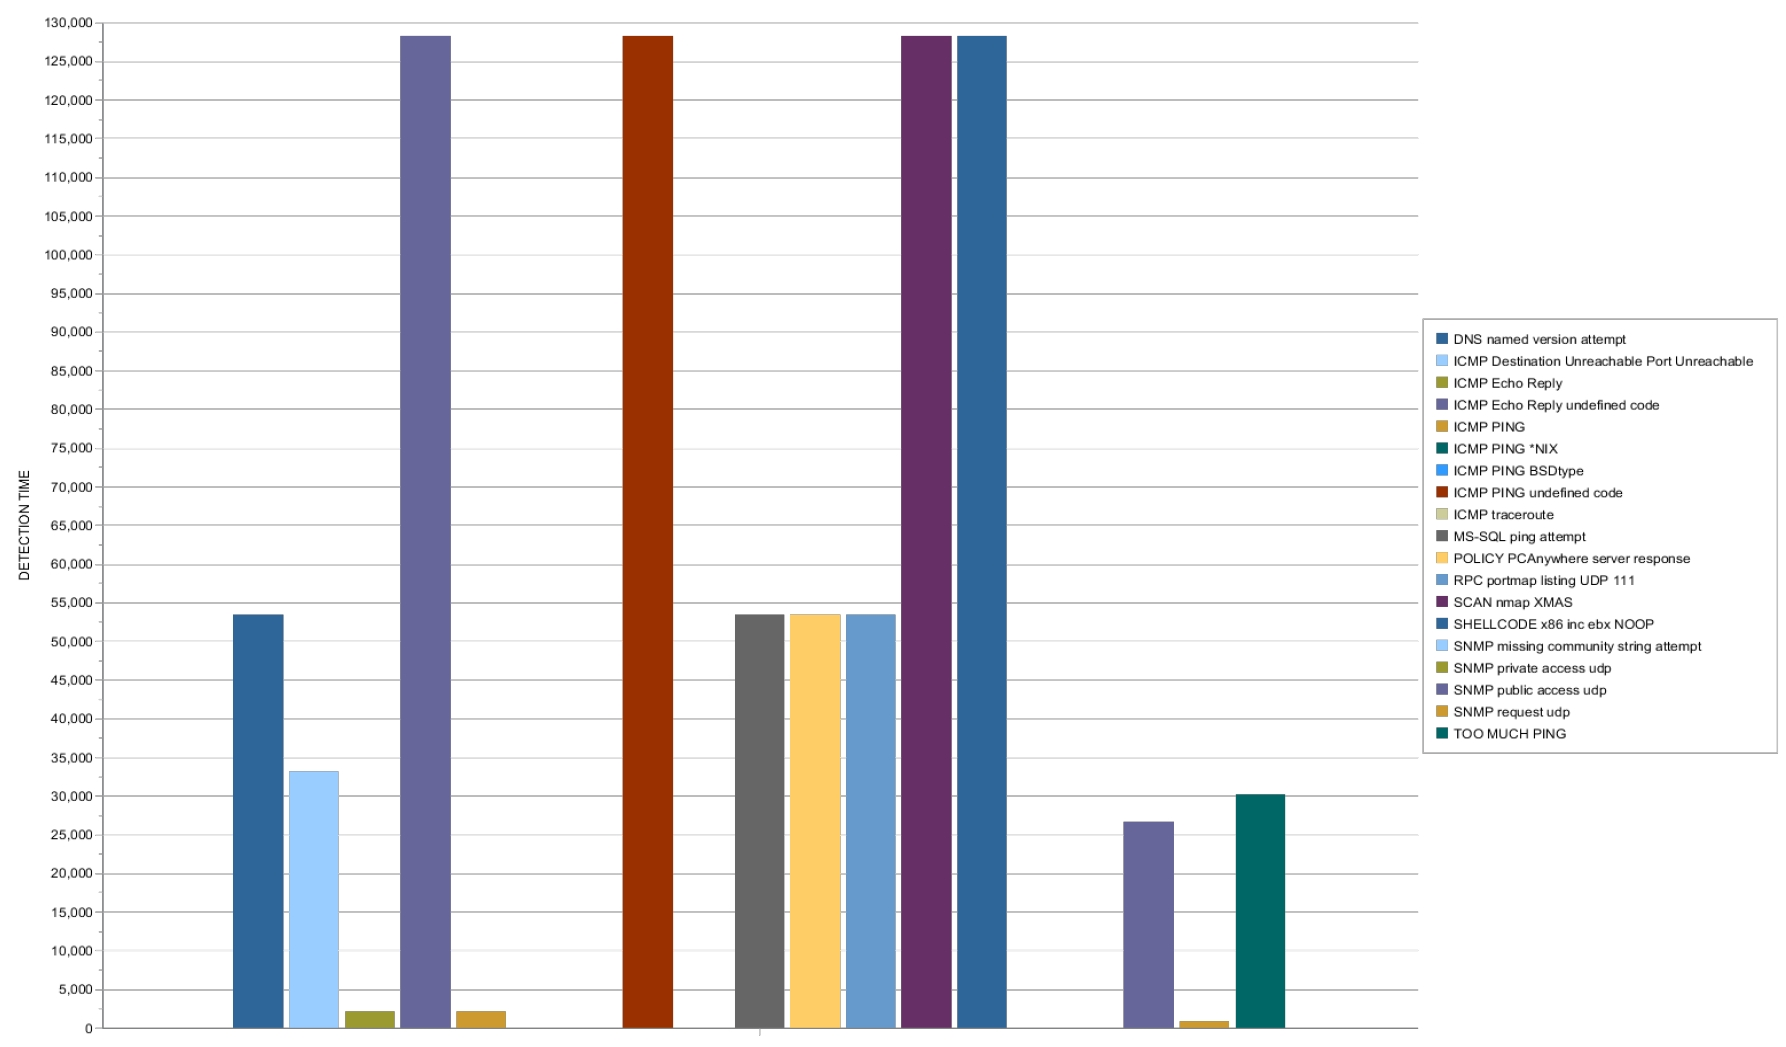
\includegraphics[scale=0.3]{figure/detection_msg.jpg}\\

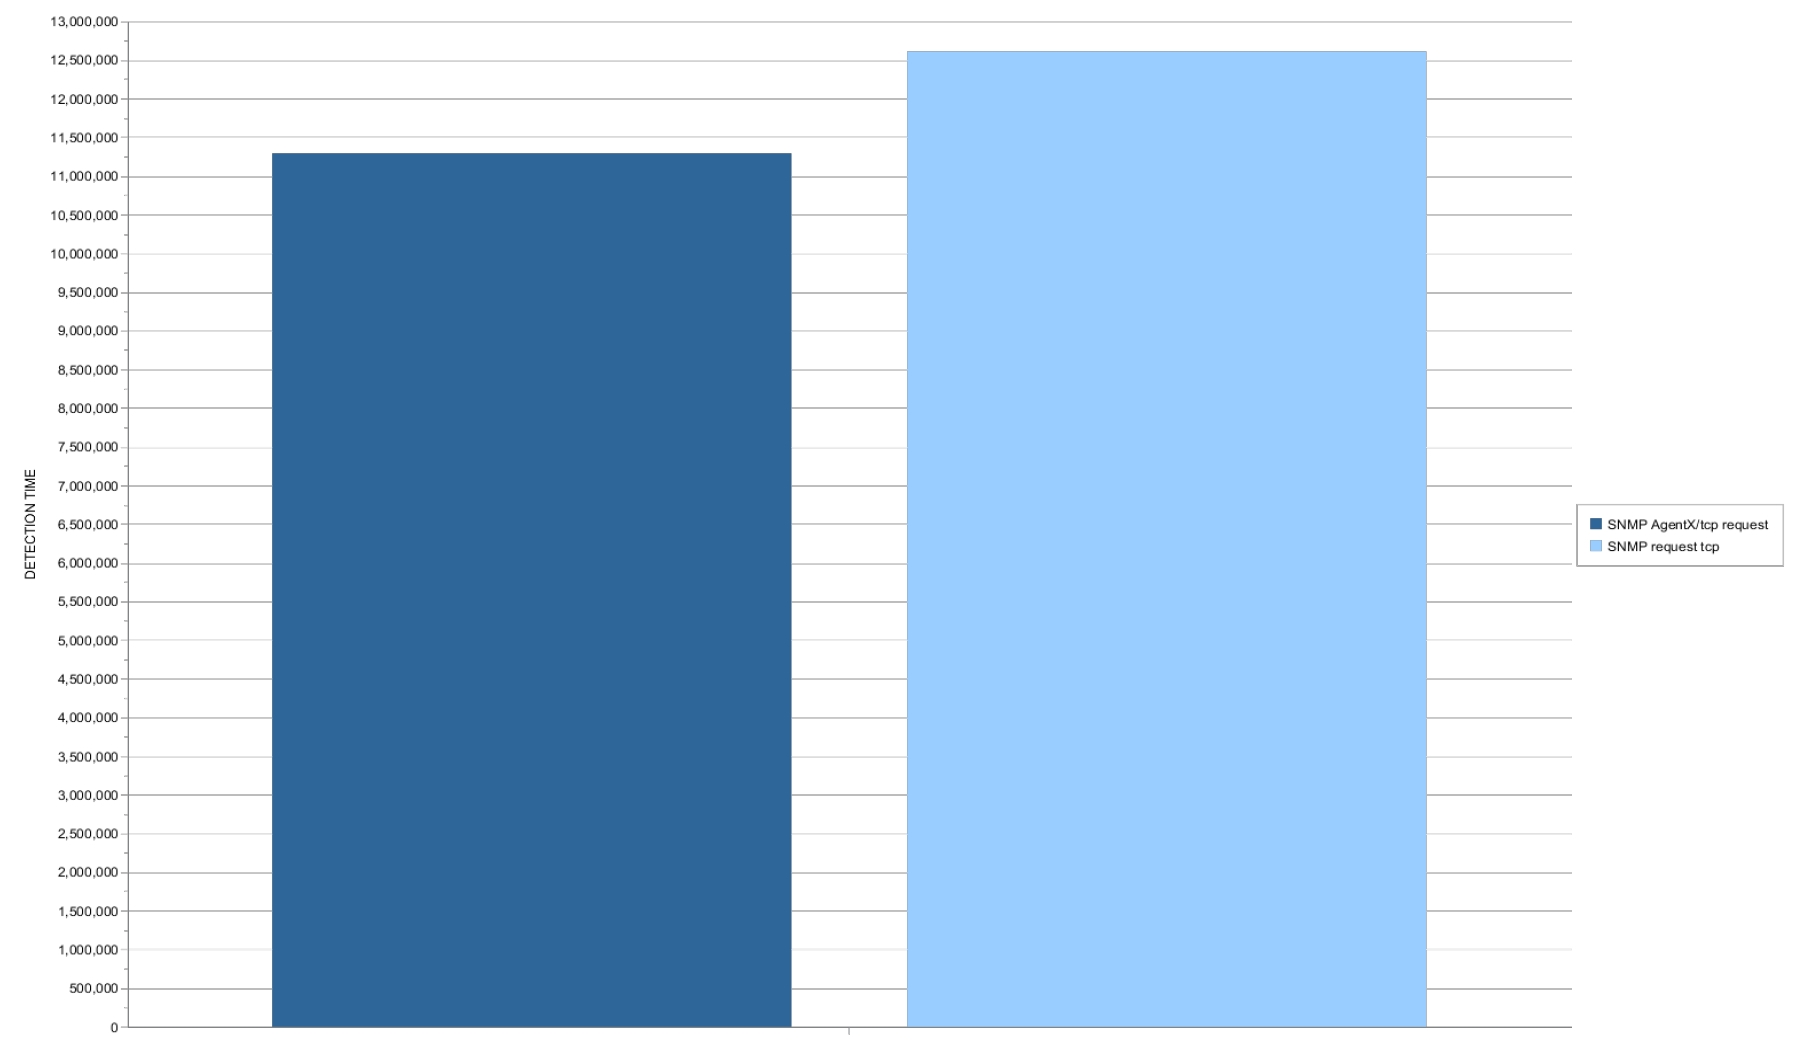
\includegraphics[scale=0.3]{figure/detection_SNMP.jpg}\\

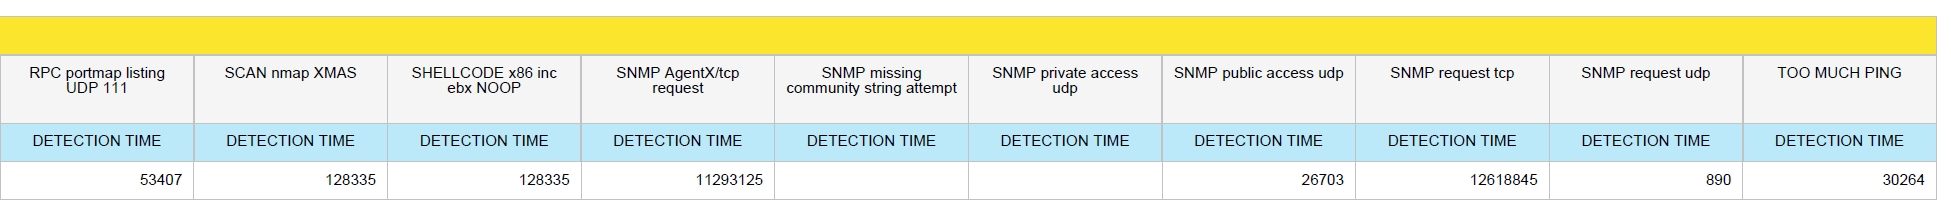
\includegraphics[scale=0.25]{figure/tabella_detection_msg_2.jpg}\\

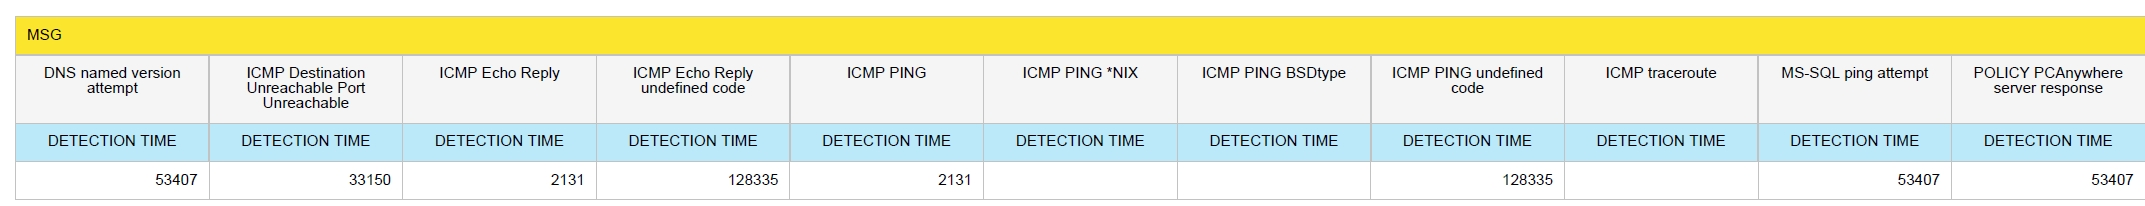
\includegraphics[scale=0.25]{figure/tabella_detection_msg_1.jpg}

	\chapter{Conclusioni} \label{chap:conclusioni}

    Concludiamo questa tesi con alcune riflessioni sul lavoro svolto.
    
    Il Progetto KT per Indico è stato sicuramente molto utile per il progetto Indico in quanto ha aggiunto molte funzionalità che prima mancavano e che certamente lo renderanno più visibile al mondo esterno, anziché esclusivamente all'interno del \ac{CERN} e dell'ambiente della fisica delle particelle.
    
    Grazie al progetto di Cloud Deployment è adesso possibile, tramite un semplice script, installare Indico su una macchina virtuale o installarlo, da remoto, su un server cloud. Inoltre, grazie allo script di gestione, è anche resa più facile all'utente la gestione dell'istanza di Indico installata su macchina virtuale, fornendo una maggior destrezza di utilizzo.
    
    Lo script fabric per le distribuzioni di Indico ha invece reso certamente la vita più facile al team di sviluppo di Indico al \ac{CERN} che adesso potranno, tramite l'invocazione di un solo comando, creare nuove distribuzioni di Indico e caricarle su un server o su GitHub in maniera completamente automatica.
    
    Il progetto di Instance Tracking si è rivelato essere il più importante tra tutti in quanto ha portato allo sviluppo di un'applicazione completamente nuova e indipendente da Indico: Cephalopod. Grazie a Cephalopod sarà adesso possibile tracciare e creare statistiche sulle istanze di Indico installate in tutto il mondo. Non solo, Cephalopod riveste un ruolo ancora più importante in quanto è utilizzabile non soltanto da Indico, ma anche da altre applicazioni web che intendono tracciare le proprie istanze, sia al \ac{CERN} che altrove.
    
    L'ultima fase del progetto, anche se non molto rilevante dal punto di vista implementativo, è invece stata molto utile in quanto ha stabilito le basi di sviluppo sul quale il team di Indico andrà a creare, in futuro, un nuovo tool per la creazione e la personalizzazione di conferenze che sarà basato sul sistema ibrido blocco-widget ed implementerà un'intuitiva interfaccia drag-and-drop.
    
    Concludendo, l'esperienza al \ac{CERN} è stata un'esperienza altamente formativa, sia dal punto di vista professionale, permettendo di studiare ed utilizzare molti strumenti e linguaggi nuovi, che umano. Infatti, oltre all'aspetto lavorativo, i 14 mesi passati a Ginevra hanno portato ad un arricchimento e ad una crescita sotto molti punti di vista, che trascendono il semplice ambito professionale.

	\appendix \chapter{Codice} 
\lstinputlisting[language=java, caption={Codice Java utilizzato per arricchire il log CSV con una serie di misure temporali derivate.}, label=lst:java]{../codice/processCSV.java}
\lstinputlisting[caption={Regola di Snort utilizzata lato attaccante per loggare i pacchetti in uscita.}, label=lst:attaccante]{../codice/ATTACCANTE.rules}
\lstinputlisting[caption={Regole di Snort utilizzate lato IDS per loggare i pacchetti in entrata e rilevare un eccessivo numero di ping.}, label=lst:ids]{../codice/IDS.rules}

\end{document}


